%% KMA — Báo cáo môn PP NCKH trong ATTT (Lớp CHAT4P). Định dạng BÁO CÁO HỌC THUẬT (một cột).
%% Biên dịch bằng Tectonic/XeLaTeX (claude-prism). Tiếng Việt qua fontspec (Latin Modern phủ dấu).
%% Cấu trúc: phần thân được tách theo chương trong thư mục sections/ và \input ở dưới.
\documentclass[12pt,a4paper]{article}

\usepackage{fontspec}
\usepackage[a4paper,margin=2.6cm]{geometry}
\usepackage{amsmath,amssymb}
\usepackage{graphicx}
\usepackage{float}
\usepackage{booktabs}
\usepackage{array}
\usepackage[table]{xcolor}
\newcolumntype{C}[1]{>{\centering\arraybackslash}p{#1}}
\newcommand{\yes}{\textcolor{green!55!black}{\checkmark}}
\newcommand{\no}{\textcolor{red!72!black}{\ensuremath{\times}}}
\usepackage{setspace}
\usepackage{caption}
\usepackage{enumitem}
\usepackage[hidelinks]{hyperref}
\usepackage{microtype}

\onehalfspacing
\captionsetup{font=small,labelfont=bf}
\setlength{\parskip}{4pt}
\renewcommand{\abstractname}{Tóm tắt}

\begin{document}

%% ===================== TRANG BÌA =====================
\begin{titlepage}
\centering
{\large BAN CƠ YẾU CHÍNH PHỦ\par}
{\large HỌC VIỆN KỸ THUẬT MẬT MÃ\par}
\vspace{0.4cm}
\vfill
{\Large\bfseries BÁO CÁO NGHIÊN CỨU\par}
\vspace{0.6cm}
{\huge\bfseries Nghiên cứu cơ chế phát hiện tấn công leo thang đặc quyền trong môi trường Multi-tenant Kubernetes dựa trên phân tích System Calls\par}
\vspace{0.6cm}
\vfill
\begin{flushright}
\begin{tabular}{@{}ll@{}}
\textbf{Học viên:} & Nguyễn Ngọc Hoài — CHAT4P006 \\
\textbf{GVHD:} & TS. Vũ Thị Vân \\
\end{tabular}
\end{flushright}
\vspace{0.5cm}
{\large Năm 2026\par}
\end{titlepage}

%% ===================== TÓM TẮT =====================
\begin{abstract}
\noindent Trong môi trường Kubernetes đa người thuê (multi-tenant), nhiều người thuê cùng chia sẻ một nhân (kernel) trên cùng một nút; do đó các tấn công leo thang đặc quyền và thoát khỏi container trở thành rủi ro trọng yếu. Các khung phát hiện bất thường dựa trên lời gọi hệ thống (system call) thu thập qua eBPF — tiêu biểu là DeSFAM — kết hợp bộ tự mã hoá biến phân (VAE) và rừng cô lập (Isolation Forest), đồng thời dùng ngưỡng động cập nhật theo trung bình trượt luỹ thừa (EMA) nhằm giảm báo động giả do hành vi lành tính trôi dạt theo thời gian. Báo cáo vận dụng phương pháp thực nghiệm ứng dụng để: (i) tái lập bộ phát hiện DeSFAM (VAE + Isolation Forest) trên tập dữ liệu thực DongTing; và (ii) kiểm định một giả thuyết đối kháng: nếu ngưỡng EMA được cập nhật \textit{vô điều kiện} — cách đọc theo nghĩa đen công thức EMA của DeSFAM — thì một ``hàng xóm gây nhiễu'' (tenant lân cận) bơm tải lành tính có thể đẩy ngưỡng toàn cục lên cao, giúp một tấn công lén lút né tránh phát hiện. Bộ phát hiện tái lập đạt AUC $=0{,}832$ (xấp xỉ DeSFAM). Phát hiện chính: khi hàng xóm gây nhiễu hoạt động mạnh, ngưỡng EMA bị đẩy lên cao đến mức để \textit{$74{,}2\%$ hoạt động của một tấn công lén lút lọt qua}, trong khi một ngưỡng cố định vẫn phát hiện được toàn bộ; nhiễu càng mạnh thì tỷ lệ bỏ sót càng cao. Đáng chú ý, với tấn công \textit{loud} (điểm bất thường rất cao), ngưỡng EMA tự bị đẩy lên \textit{ngay cả khi không có} hàng xóm gây nhiễu — do chính các cửa sổ tấn công bơm ngưỡng — cho thấy lỗ hổng còn nằm ở \textit{chính quy tắc cập nhật ngưỡng}, không chỉ ở môi trường đa người thuê. Ngược lại, dạng cập nhật \textit{có điều kiện} mà chính Algorithm 2 của DeSFAM đặc tả (chỉ cập nhật ngưỡng trên cửa sổ \textit{không} bị báo động) miễn nhiễm hoàn toàn ($0\%$). Đây là một nghiên cứu cơ chế trên điểm bất thường của DongTing; việc kiểm chứng trực tuyến trên cụm Kubernetes với Tetragon và tấn công leo thang đặc quyền thực là hướng phát triển tiếp theo. Báo cáo qua đó vạch ra một \textit{sự thiếu nhất quán} trong đặc tả của DeSFAM — công thức EMA (vô điều kiện) so với Algorithm 2 (có điều kiện) — và chứng minh rằng quy tắc cập nhật có điều kiện của Algorithm 2 là \textit{thiết yếu về an ninh}, chứ không chỉ để giảm báo động giả.

\medskip
\noindent\textbf{Từ khoá:} phát hiện xâm nhập, lời gọi hệ thống, eBPF, Kubernetes, leo thang đặc quyền, phát hiện bất thường, ngưỡng thích nghi, né tránh đối kháng.
\end{abstract}

\newpage
\tableofcontents
\newpage

%% ===================== PHẦN THÂN (tách theo chương) =====================
%% ===================== 1. GIỚI THIỆU =====================
\section{Giới thiệu}

\subsection{Bối cảnh}
Containerisation và Kubernetes (K8s) là nền tảng triển khai phần mềm hiện đại nhờ tính nhẹ và khả năng co giãn. Khác với máy ảo, các container trên cùng một node chia sẻ chung Linux kernel; ranh giới cô lập (isolation boundary) chỉ dựa trên các kernel primitive như namespace, cgroup, capability và seccomp. Một thoả hiệp tại một container — thông qua privilege escalation hoặc khai thác lỗ hổng kernel — có thể vượt ranh giới này để lan sang tenant khác hoặc chiếm quyền điều khiển node~\cite{crosscontainer2023,ebpfguard2026}. Trong mô hình multi-tenant, nơi các tenant không tin cậy lẫn nhau cùng tồn tại, đây là một rủi ro hệ trọng (minh hoạ ở Hình~\ref{fig:threat}).

\begin{figure}[ht]
\centering
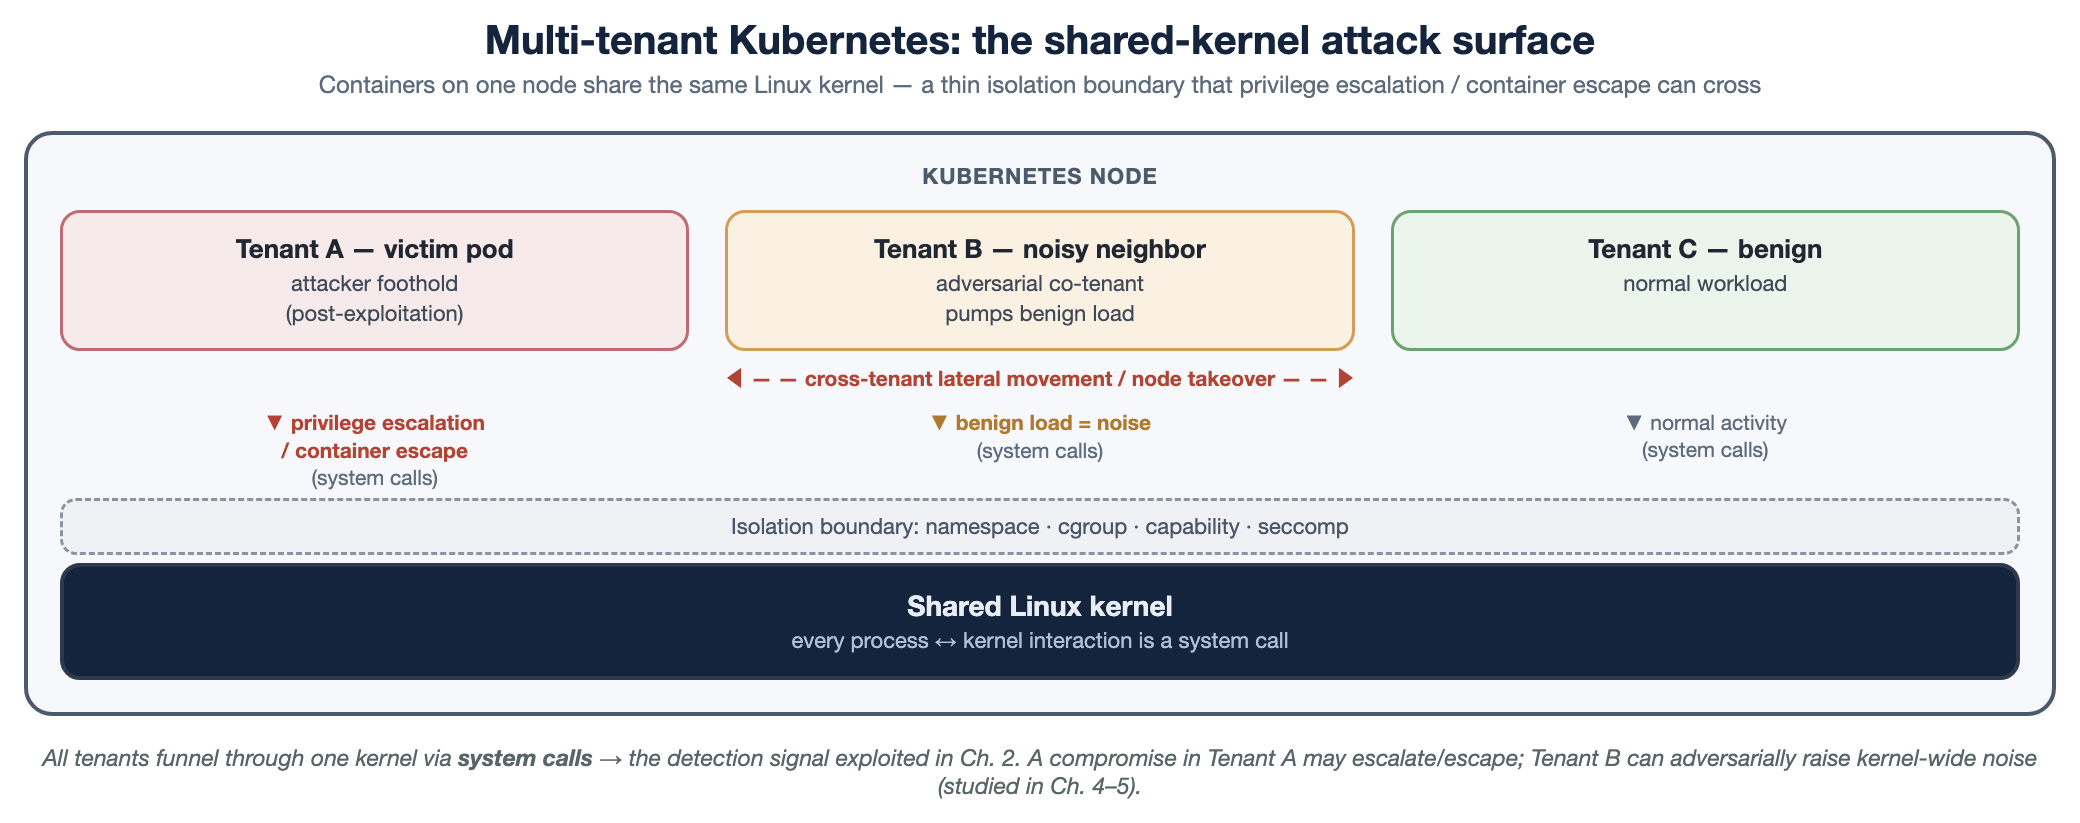
\includegraphics[width=\textwidth]{figures/fig_threat.png}
\caption{Bề mặt tấn công shared-kernel trong Multi-tenant Kubernetes.}
\label{fig:threat}
\end{figure}

Do mọi tương tác giữa tiến trình và kernel đều đi qua system call, đây là tín hiệu trung tâm của \textit{host-based intrusion detection} (HIDS — phát hiện xâm nhập trên máy chủ)~\cite{forrest1996sense,creech2014semantic,liu2018hids,bridges2019hostdata}. Công nghệ eBPF giúp thu thập system call ở mức kernel với chi phí thấp, thúc đẩy một thế hệ công cụ runtime security cho cloud-native~\cite{syairozi2025ebpfcompare,safebpf2024,hu2026eids}; trong đó \textit{DeSFAM} là một đại diện kết hợp AI mà báo cáo này lấy làm hệ cơ sở (base). Nền tảng và các công trình liên quan được trình bày chi tiết ở Chương~\ref{sec:related}.

\subsection{Động lực nghiên cứu}
DeSFAM và biến thể federated FedMon~\cite{desfam_original,fedmon2025} sử dụng cơ chế \textit{ngưỡng động} (adaptive threshold): ngưỡng cảnh báo được tự động nâng lên khi mức độ hoạt động của hệ thống gia tăng, nhằm hạn chế báo động giả phát sinh từ benign behavioral drift (sự trôi dạt hành vi lành tính theo thời gian). Mặc dù cùng hướng tới môi trường multi-tenant, cả hai chỉ được đánh giá trong điều kiện vận hành lành tính, chưa xét đến sự hiện diện của một đối thủ.

Chính cơ chế thích nghi này lại làm nảy sinh một nghịch lý an ninh. Trên hạ tầng public cloud, nơi các tenant dùng chung tài nguyên, một co-tenant không đáng tin có thể \textit{chủ động} sinh ra tải nền có mức bất thường cao — hiện tượng noisy neighbor (hàng xóm gây nhiễu) — kéo ngưỡng động lên cao hơn mức phản ánh rủi ro thực sự. Một tấn công có tín hiệu thấp (stealthy) khi đó rơi xuống dưới ngưỡng và thoát khỏi phạm vi phát hiện. Như vậy, cơ chế vốn được thiết kế để giảm báo động giả lại trở thành một attack surface (bề mặt tấn công). Mức độ nguy hiểm phụ thuộc vào một chi tiết tưởng nhỏ: ngưỡng được cập nhật \textit{vô điều kiện} (sau mọi cửa sổ) hay \textit{có điều kiện} (chỉ trên cửa sổ không bị gắn cờ) — và chính đặc tả của DeSFAM lại không nhất quán về điểm này (Mục~\ref{ss:desfam}). Báo cáo kiểm chứng trực tiếp giả thuyết này (các khoảng trống nghiên cứu tại Mục~\ref{ss:gap}).

\subsection{Câu hỏi nghiên cứu và nội dung}
Báo cáo hướng tới hai câu hỏi nghiên cứu:
\begin{description}[leftmargin=1.4cm,style=nextline]
\item[RQ1] Bộ phát hiện kiểu DeSFAM đạt năng lực phát hiện ở mức nào đối với tấn công privilege escalation (leo thang đặc quyền) và container escape (thoát container) trên dữ liệu thực, đo bằng recall, precision và AUC?
\item[RQ2] (trọng tâm) Khi ngưỡng EMA được cập nhật \textit{vô điều kiện}, một noisy neighbor bơm tải lành tính có làm nâng ngưỡng và qua đó tạo điều kiện cho evasion (né tránh phát hiện) hay không; mức độ biến thiên ra sao theo cường độ nhiễu và loại tấn công; và dạng cập nhật \textit{có điều kiện} của Algorithm 2 (DeSFAM) có loại bỏ được lỗ hổng này không?
\end{description}

Tương ứng, nội dung nghiên cứu gồm ba phần: (i) tái lập bộ phát hiện kiểu DeSFAM và đánh giá năng lực phát hiện trên tập dữ liệu thực DongTing (RQ1); (ii) phát biểu chính xác, kiểm định và định lượng giả thuyết \textit{threshold-inflation evasion} — kẻ tấn công lợi dụng việc ngưỡng động bị nâng để né tránh phát hiện — trên anomaly score thực, có kiểm định thống kê, đồng thời chỉ ra rằng dạng cập nhật \textit{vô điều kiện} tự nâng ngưỡng ngay cả khi không có đối thủ (self-inflation); và (iii) chỉ ra \textit{sự thiếu nhất quán} giữa công thức EMA (vô điều kiện) và Algorithm 2 (có điều kiện) của DeSFAM, và kiểm chứng rằng dạng cập nhật có điều kiện của Algorithm 2 vô hiệu hoá hoàn toàn vector tấn công ($0\%$) — tức là một biện pháp \textit{thiết yếu về an ninh}, không chỉ để giảm báo động giả (RQ2).

\subsection{Cấu trúc báo cáo}
Phần còn lại của báo cáo được tổ chức như sau: Mục~\ref{sec:related} — cơ sở lý thuyết và công trình liên quan; Mục~\ref{sec:method} — phương pháp luận; Mục~\ref{sec:setup} — thiết lập thực nghiệm; Mục~\ref{sec:results} — kết quả; Mục~\ref{sec:discuss} — thảo luận và threat to validity; Mục~\ref{sec:concl} — kết luận; Phụ lục~\ref{sec:repro} — hướng dẫn tái lập.

% !TeX root = ../main.tex
%% ===================== 2. CƠ SỞ & RELATED WORK =====================
\section{Cơ sở lý thuyết và Công trình liên quan}\label{sec:related}
Chương này trình bày nền tảng phát hiện xâm nhập dựa trên lời gọi hệ thống và công nghệ eBPF (Mục~\ref{ss:hids}); hệ cơ sở DeSFAM cùng cơ chế ngưỡng động (Mục~\ref{ss:desfam}); và từ đó tổng hợp các khoảng trống nghiên cứu mà báo cáo hướng tới (Mục~\ref{ss:gap}).

\subsection{Phát hiện xâm nhập dựa trên lời gọi hệ thống và eBPF}\label{ss:hids}
Phát hiện xâm nhập trên máy chủ (host-based intrusion detection, HIDS) dựa trên lời gọi hệ thống (system call) có nền tảng từ mô hình self/non-self~\cite{forrest1996sense}: một tiến trình lành tính sinh ra phân phối và trình tự system call tương đối ổn định, nên độ lệch khỏi mô hình ``bình thường'' là dấu hiệu của xâm nhập. Hướng tiếp cận này về sau được mở rộng bằng các đặc trưng ngữ nghĩa trên chuỗi system call~\cite{creech2014semantic} và được hệ thống hoá trong nhiều khảo sát~\cite{liu2018hids,bridges2019hostdata}, vốn nêu ba thách thức cốt lõi: giảm tỷ lệ báo động giả (false positive rate, FPR), bảo đảm hiệu năng, và chịu được behavioral drift (sự trôi dạt hành vi lành tính theo thời gian). Tập dữ liệu \textit{DongTing}~\cite{dongting2023} — gồm 18.966 chuỗi system call có nhãn, thu thập trên hơn 200 phiên bản kernel — là dữ liệu nền của báo cáo.

Trong môi trường container, công nghệ eBPF cho phép quan sát system call ngay tại mức kernel một cách an toàn và chi phí thấp (Hình~\ref{fig:ebpf}), tạo nền tảng cho một thế hệ công cụ runtime security; SafeBPF~\cite{safebpf2024} thậm chí cô lập chính các chương trình eBPF (chi phí $0$--$7\%$). Trên nền eBPF, hai hướng phát hiện song song tồn tại. Hướng \textit{dựa trên luật} (rule-based) — Falco, Tetragon, Tracee — đạt độ phát hiện đầy đủ với độ trễ thấp ($\sim 0{,}4$--$1{,}6$\,s) trên các kịch bản đã biết, nhưng phụ thuộc danh sách luật cố định nên dễ bỏ sót biến thể mới~\cite{syairozi2025ebpfcompare}. Hướng \textit{dựa trên học máy} (ML-based) nhằm phát hiện cả tấn công chưa biết: eBPF-Guard~\cite{ebpfguard2026} giám sát đa tầng để phát hiện container escape; eBPF-PATROL~\cite{ebpfpatrol2025} nhận diện hành vi vượt quyền; EIDS~\cite{hu2026eids} hướng tới IDS đám mây hiệu năng cao; Kotenko \textit{và cộng sự}~\cite{kotenko2025containerae} dùng autoencoder trên histogram system call; LIGHT-HIDS~\cite{lighthids2025} dùng novelty detection nhẹ; và các mô hình chuỗi (Transformer, LLM) được tổng hợp trong~\cite{translmidssurvey}, vốn nhấn mạnh rằng phát hiện \textit{trực tuyến} bằng mô hình nặng vẫn là thách thức về độ trễ. DeSFAM — hệ cơ sở của báo cáo — thuộc hướng học máy này (Mục~\ref{ss:desfam}).

\begin{figure}[ht]
\centering
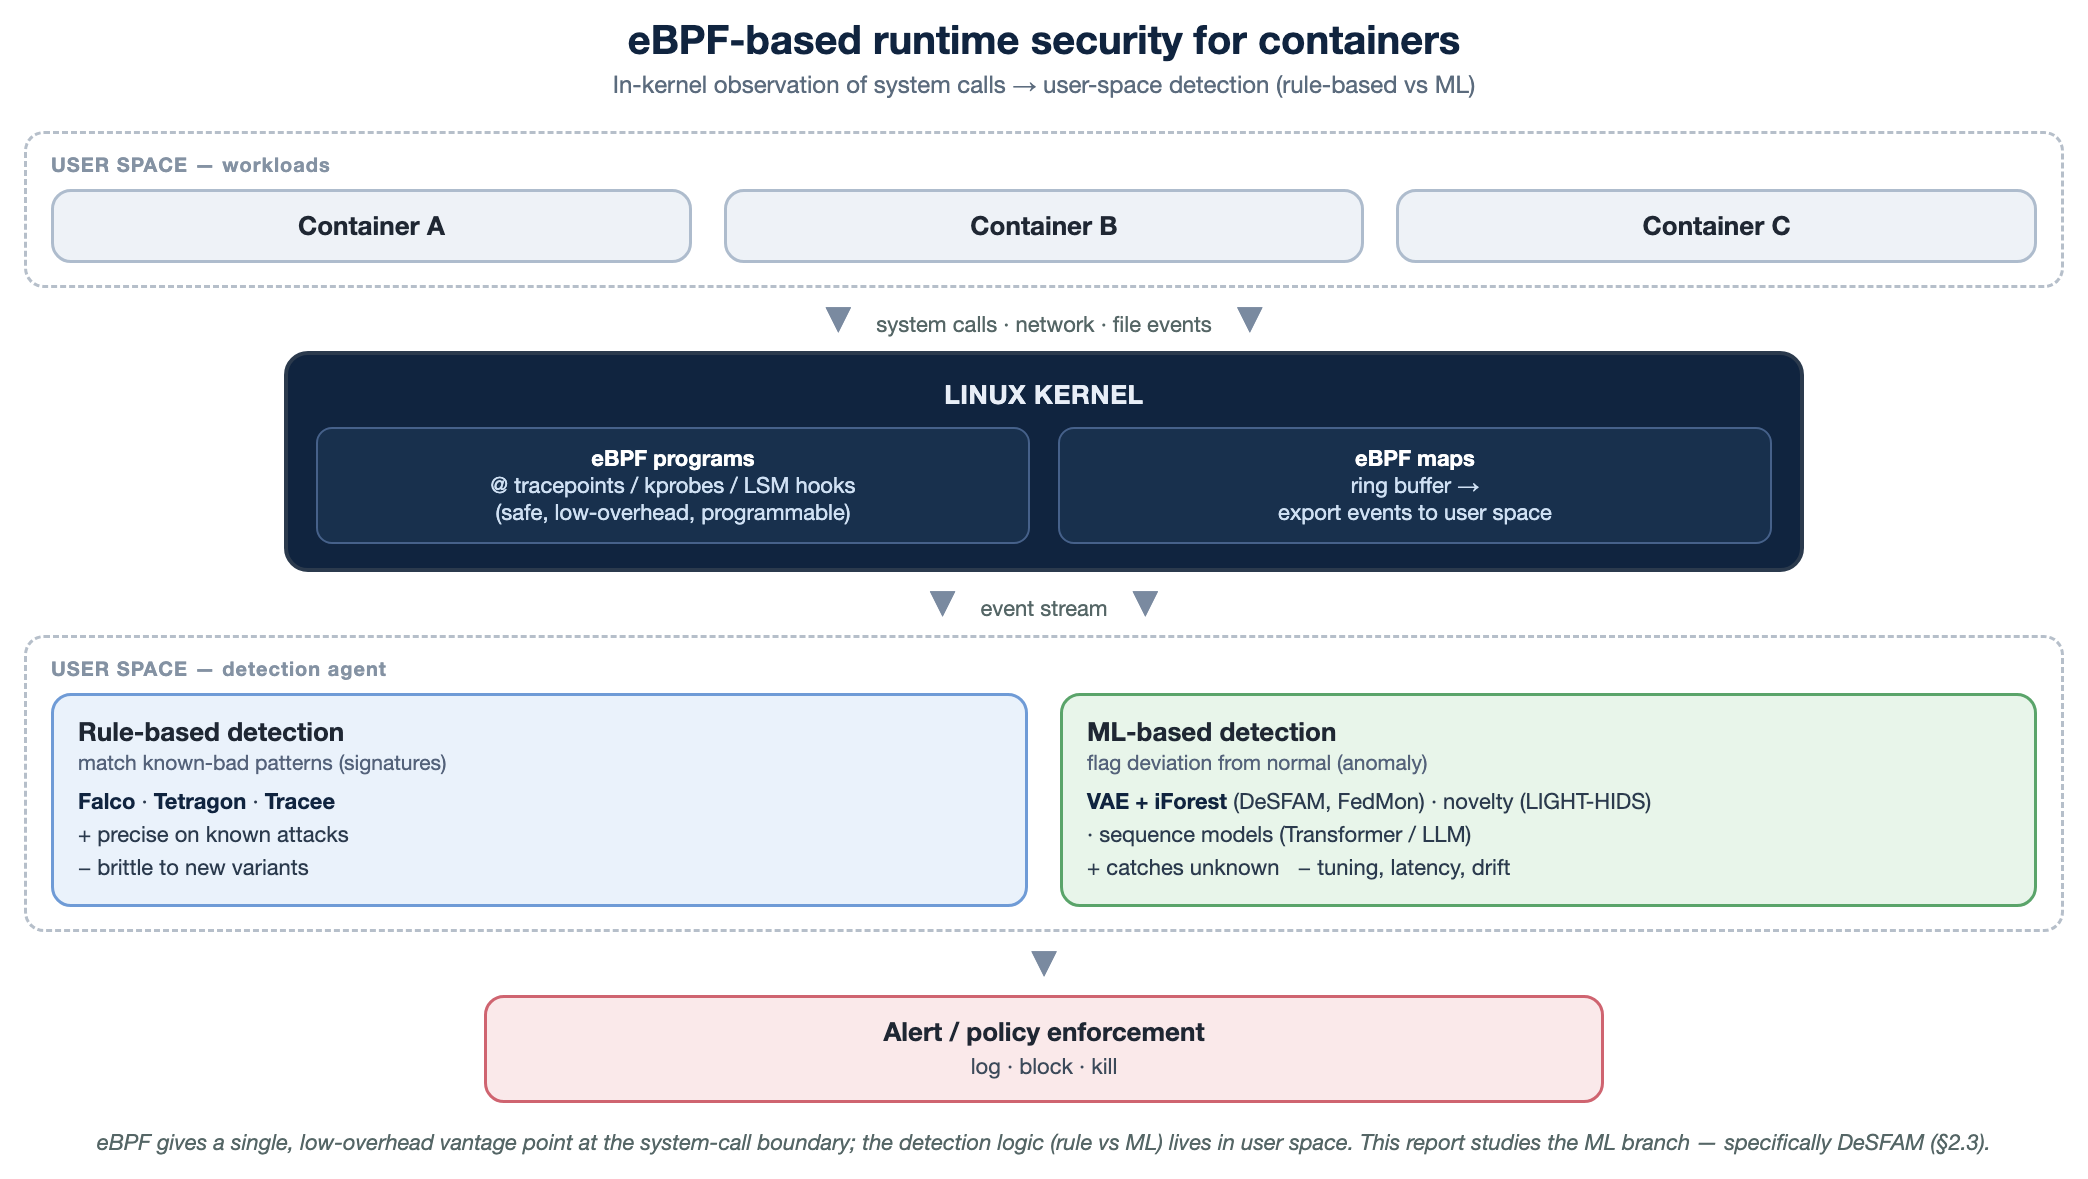
\includegraphics[width=\textwidth]{figures/fig_ebpf_runtime.png}
\caption{Quan sát system call qua eBPF và hai hướng phát hiện (rule-based và ML).}
\label{fig:ebpf}
\end{figure}

\subsection{DeSFAM và cơ chế ngưỡng động}\label{ss:desfam}
DeSFAM~\cite{desfam_original} là khung kết hợp eBPF và học máy cho anomaly detection ở runtime container, được báo cáo lựa chọn làm hệ cơ sở. Thành phần lõi của nó — \textit{SyscallAD} — vận hành theo ba bước. Thứ nhất, mỗi \textit{sliding window} (cửa sổ trượt) các system call được biểu diễn thành một vector đặc trưng gồm tần suất theo nhóm chức năng, đặc trưng thời gian, và mức độ khớp với mẫu hành vi lành tính. Thứ hai, vector này được chấm điểm bất thường bằng một \textit{ensemble} gồm Variational Autoencoder (VAE) và Isolation Forest, cả hai huấn luyện theo chế độ \textit{normal-only} (chỉ trên dữ liệu lành tính) và hợp nhất theo trọng số $0{,}7/0{,}3$. Thứ ba, quyết định cảnh báo dựa trên một \textit{ngưỡng động}: ngưỡng được khởi tạo tại phân vị $99{,}5$ của phân phối điểm bất thường lành tính, rồi cập nhật theo exponential moving average (EMA).

Một điểm mấu chốt cho báo cáo này là \textbf{bản thân DeSFAM mô tả quy tắc cập nhật ngưỡng theo hai cách không nhất quán}. Phần lời quanh công thức (3) viết rằng ngưỡng ``được cập nhật \textit{sau mỗi cửa sổ}'' — đọc theo nghĩa đen là cập nhật \textit{vô điều kiện}. Tuy nhiên, đặc tả hình thức trong \textit{Algorithm 2} của DeSFAM~\cite{desfam_original} lại đặt phép cập nhật trong nhánh \texttt{else}: nếu $A(W_i)>T$ thì gắn cờ (\textit{không} cập nhật ngưỡng), \textit{ngược lại} mới cập nhật $T \leftarrow \max(T_{\min}, \beta T + (1-\beta)A)$. Tức Algorithm 2 \textbf{chỉ cập nhật trên cửa sổ không bị gắn cờ} — cập nhật \textit{có điều kiện}. Sự mơ hồ giữa lời văn (vô điều kiện) và thuật toán (có điều kiện) chính là điểm mà báo cáo khai thác và làm rõ: như sẽ thấy ở Mục~\ref{sec:results}, khác biệt này có \textit{hệ quả an ninh} trực tiếp. Chi tiết hình thức hoá ở Mục~\ref{sec:method}; minh hoạ cơ chế ở Hình~\ref{fig:desfam}. Biến thể federated FedMon~\cite{fedmon2025} kế thừa kiến trúc này và tự thừa nhận hạn chế trước workload \textit{non-IID} (dị thể giữa các tenant) — cho thấy nhiễu đa người thuê là một vấn đề có thật đối với họ DeSFAM; báo cáo này khảo sát chính nhiễu đó dưới \textit{góc độ đối kháng}, chứ không nhằm giải quyết khía cạnh độ chính xác của học liên kết.

\begin{figure}[ht]
\centering
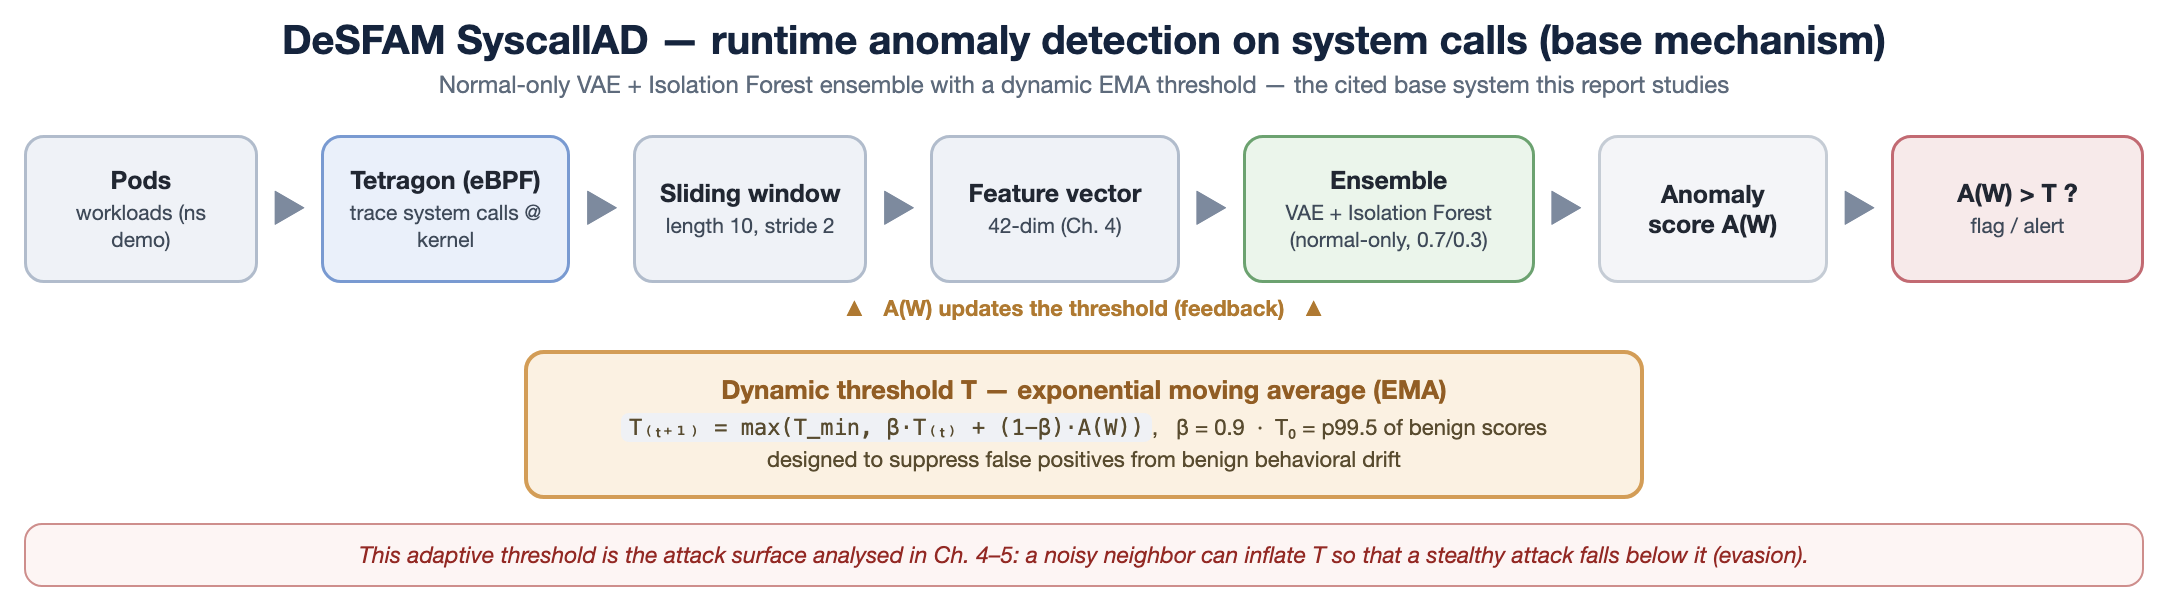
\includegraphics[width=\textwidth]{figures/fig_desfam.png}
\caption{Cơ chế phát hiện của DeSFAM SyscallAD (hệ cơ sở).}
\label{fig:desfam}
\end{figure}

\subsubsection{Vai trò của VAE và Isolation Forest}
Hai mô hình được lựa chọn vì \textit{bổ trợ} cho nhau và đều huấn luyện được theo chế độ \textit{normal-only} — phù hợp với thực tế an ninh, nơi mẫu tấn công hiếm, đa dạng và khó thu thập đầy đủ; do đó việc chỉ học từ hành vi lành tính là khả thi hơn so với học có giám sát cần nhãn tấn công.

\textbf{Variational Autoencoder (VAE)} là một mô hình sinh (generative) học cách nén rồi tái tạo dữ liệu qua một không gian ẩn (latent space) có cấu trúc xác suất. Khi chỉ huấn luyện trên hành vi lành tính, VAE tái tạo tốt các cửa sổ bình thường nhưng tái tạo kém các cửa sổ bất thường; vì vậy \textit{sai số tái tạo} (reconstruction error) lớn được dùng làm điểm bất thường. Ưu điểm là nắm bắt được cấu trúc phi tuyến và phân phối tinh vi của hành vi bình thường; hạn chế là nhạy với tính đại diện của dữ liệu huấn luyện và có thể gặp posterior collapse.

\textbf{Isolation Forest} là một tập hợp cây phân tách ngẫu nhiên: điểm bất thường thường bị \textit{cô lập} chỉ sau vài bước chia, nên độ dài đường đi (path length) ngắn tương ứng với mức bất thường cao. Ưu điểm là nhẹ, không giả định phân phối dữ liệu, ổn định và hiệu quả trên không gian nhiều chiều; hạn chế là chỉ phản ánh mức ngoại lai \textit{toàn cục}, kém tinh tế hơn VAE trước các sai lệch cục bộ.

\textbf{Vì sao kết hợp (ensemble $0{,}7/0{,}3$).} VAE mạnh ở việc mô hình hoá manifold của dữ liệu bình thường nhưng kém ổn định; Isolation Forest thô hơn song bền vững và chi phí thấp. Hợp nhất hai điểm số đã chuẩn hoá theo trọng số $0{,}7$ (VAE) và $0{,}3$ (Isolation Forest) giúp giảm điểm yếu của từng mô hình và cho điểm bất thường ổn định hơn so với khi dùng riêng lẻ. Trọng số $\alpha=0{,}7$ không phải lựa chọn tuỳ ý: nhóm tác giả DeSFAM xác định nó qua phân tích độ nhạy trên $\alpha\in\{0{,}0;\,0{,}25;\,0{,}5;\,0{,}7;\,0{,}85;\,1{,}0\}$, với F1 và AUC đạt đỉnh tại $\alpha=0{,}7$~\cite{desfam_original}.

Bảng~\ref{tab:related} định vị DeSFAM cùng các hướng phát hiện liên quan.

\begin{table}[ht]
\caption{So sánh các hướng phát hiện trên cloud/K8s.}
\label{tab:related}
\centering
\renewcommand{\arraystretch}{1.35}
\begin{tabular}{@{}p{2.9cm}p{3.4cm}C{1.6cm}C{1.7cm}C{1.9cm}@{}}
\toprule
Công trình & Phương pháp & Ngưỡng động & Đa người thuê & Đánh giá đối kháng \\
\midrule
DeSFAM~\cite{desfam_original}             & VAE + iForest          & \yes\,(EMA) & \yes$^\dagger$ & \no \\
FedMon~\cite{fedmon2025}                  & VAE + iForest (FL)     & \yes\,(EMA) & \yes$^\dagger$ & \no \\
Rule-based~\cite{syairozi2025ebpfcompare} & Falco/Tetragon/Tracee  & \no         & \no            & \no \\
Kotenko~\cite{kotenko2025containerae}     & Autoencoder            & \no         & \no            & \no \\
Báo cáo này                               & VAE + iForest (DeSFAM) & \yes\,(EMA) & \yes           & \yes \\
\bottomrule
\end{tabular}
\par\smallskip{\footnotesize \yes\,= có · \no\,= không · $\dagger$\,= có hỗ trợ nhưng chưa kiểm thử dưới điều kiện thù địch.}
\end{table}

\subsection{Khoảng trống nghiên cứu}\label{ss:gap}
Khảo sát ở các Mục~\ref{ss:hids}--\ref{ss:desfam} làm nổi bật hai khoảng trống nghiên cứu chính:
\begin{enumerate}[leftmargin=1.5cm,label=(\roman*)]
\item \textbf{Tác động của nhiễu đa người thuê.} Ảnh hưởng của workload non-IID giữa các tenant lên độ nhạy của bộ phát hiện chưa được định lượng một cách hệ thống — đúng hạn chế mà FedMon~\cite{fedmon2025} tự thừa nhận.
\item \textbf{Hệ quả an ninh của cập nhật ngưỡng vô điều kiện.} Tác động an ninh khi một bộ phát hiện cập nhật ngưỡng thích nghi \textit{vô điều kiện} — như cách đọc theo nghĩa đen công thức (3) của DeSFAM, trái với Algorithm 2 — chưa được định lượng. Nói rộng hơn, khả năng một kẻ tấn công \textit{chủ động} lợi dụng cơ chế tự cập nhật ngưỡng còn ít được khảo sát hệ thống trong runtime container security; mọi đánh giá thuộc họ DeSFAM (Bảng~\ref{tab:related}) đều thực hiện trong điều kiện không thù địch.
\end{enumerate}
Báo cáo tập trung lấp hai khoảng trống này (RQ2); việc tái lập và đánh giá năng lực bộ phát hiện (RQ1) — bao gồm cả phân tích tách theo từng loại tấn công — cung cấp nền tảng cần thiết để khảo sát chúng.

%% ===================== 3. PHƯƠNG PHÁP =====================
\section{Phương pháp luận}\label{sec:method}

\subsection{Loại hình và thiết kế nghiên cứu}
Báo cáo áp dụng loại hình \textit{Applied Experimentation} (thực nghiệm ứng dụng) theo Edgar \& Manz~\cite{edgarmanz2017}: tái lập một cơ chế đã công bố, rồi thao tác một biến độc lập (independent variable) trong điều kiện kiểm soát để kiểm định một giả thuyết có thể bác bỏ. Ở đây, biến độc lập là \textit{cường độ nhiễu} của noisy neighbor; cơ chế phát hiện được giữ cố định (ceteris paribus). Việc đối chứng dynamic threshold với fixed threshold \textit{trên cùng một dòng dữ liệu} cho phép quy kết nhân quả: evasion (nếu có) đến từ \textit{cơ chế ngưỡng}, không phải do nhiễu làm méo tín hiệu.

\subsection{Giả thuyết nghiên cứu}
\begin{description}[leftmargin=1.2cm,style=nextline]
\item[H0] Cường độ nhiễu không ảnh hưởng đến recall, FPR hay giá trị EMA threshold.
\item[H1a] Tăng cường độ nhiễu làm \textit{giảm recall} và/hoặc tăng FPR một cách đơn điệu, có ý nghĩa thống kê.
\item[H1b] Nhiễu đẩy EMA threshold $T_{\text{EMA}}$ lên cao, khiến tấn công stealthy bị bỏ sót dưới EMA \textit{nhiều hơn hẳn} so với fixed threshold trên cùng dữ liệu — tức evasion bắt nguồn \textit{từ cơ chế ngưỡng}.
\end{description}

\subsection{Cơ chế ngưỡng EMA và cách ngưỡng thay đổi theo thời gian}
DeSFAM đặc tả việc cập nhật ngưỡng theo EMA bằng công thức:
\begin{equation}
T_{t+1} = \max\!\big(T_{\min},\; \beta\,T_t + (1-\beta)\,A(W_i)\big),\quad \beta=0{,}9,
\label{eq:ema}
\end{equation}
với anomaly score ensemble $A(W_i)=0{,}7\,A_{\text{VAE}}(W_i)+0{,}3\,A_{\text{iForest}}(W_i)$; một cửa sổ bị gắn cờ (flagged) khi $A(W_i)>T$. Như đã nêu ở Mục~\ref{ss:desfam}, đặc tả của DeSFAM mơ hồ giữa hai dạng cập nhật: phần lời quanh công thức~\eqref{eq:ema} đọc theo nghĩa đen là \textit{vô điều kiện}, còn Algorithm 2 lại là \textit{có điều kiện}. Báo cáo tách bạch và đánh giá ba chính sách trên \textit{cùng} dòng anomaly score:
\begin{itemize}[leftmargin=1.2cm]
\item \texttt{fixed}: $T=T_{op}$ cố định (đối chứng, không thích ứng);
\item \texttt{ema\_uncond} (\textit{unconditional} — cập nhật vô điều kiện): triển khai theo \textit{nghĩa đen} phần lời của công thức~\eqref{eq:ema} (``cập nhật sau mỗi cửa sổ''), tức cập nhật ở \textit{mọi} cửa sổ;
\item \texttt{ema\_cond} (\textit{conditional} — cập nhật có điều kiện): \textit{đúng theo Algorithm 2 của DeSFAM}~\cite{desfam_original} — chỉ cập nhật trên cửa sổ không bị gắn cờ ($A\le T$).
\end{itemize}

Báo cáo dùng ba mức ngưỡng, đặt theo phân vị của điểm bất thường lành tính; cần phân biệt rõ phần \textit{nguyên bản} của DeSFAM với phần là \textit{lựa chọn của báo cáo} (Bảng~\ref{tab:thresholds}). Giá trị cụ thể được hiệu chuẩn trên tập calibration ở Mục~\ref{sec:setup}.

\begin{table}[ht]
\caption{Ba mức ngưỡng dùng trong báo cáo và nguồn gốc của chúng.}
\label{tab:thresholds}
\centering
\begin{tabular}{@{}l l l p{5.4cm}@{}}
\toprule
\textbf{Ký hiệu} & \textbf{Đặt tại} & \textbf{Nguồn} & \textbf{Vai trò} \\
\midrule
$T_0$      & p99,5 & DeSFAM & Ngưỡng khởi tạo nguyên bản; rất khắt khe (recall thấp). \\
$T_{op}$   & p95   & Báo cáo & Operating point (FPR $\approx 5\%$); ngưỡng cố định của \texttt{fixed} và điểm xuất phát của EMA. \\
$T_{\min}$ & p50   & Báo cáo$^{\ast}$ & Sàn dưới của EMA (ngưỡng không tụt xuống dưới mức này). \\
\bottomrule
\end{tabular}
\par\smallskip{\footnotesize $T_0$, cơ chế EMA ($\beta=0{,}9$) và việc có sàn $T_{\min}$ là nguyên bản DeSFAM. $^{\ast}$DeSFAM đặt $T_{\min}=0{,}5$ \textit{cố định}; do điểm bất thường của ensemble ở đây đã được z-hoá (không nằm trong $[0,1]$), báo cáo dùng phân vị 50 làm mức tương ứng.}
\end{table}

Trong ba chính sách, \texttt{ema\_cond} chính là Algorithm 2 của DeSFAM (Mục~\ref{ss:desfam}) — không phải đề xuất của báo cáo; \texttt{ema\_uncond} là cách đọc theo nghĩa đen công thức~\eqref{eq:ema}. Chỉ \texttt{fixed} và operating point $T_{op}=$\,p95 là lựa chọn của báo cáo, có lý do phương pháp luận rõ ràng. \texttt{fixed} đóng vai trò \textit{nhóm đối chứng} để quy kết nhân quả (Mục~\ref{sec:method}). Về $T_{op}$: tại $T_0=$\,p99,5 nguyên bản, detector chỉ đạt recall $0{,}006$ trên DongTing — gần như không bắt được gì \textit{trước cả khi} có nhiễu, nên không có gì để ``mất'' và evasion không quan sát được. Vì vậy báo cáo chọn operating point p95 nhằm tạo một chế độ vận hành mà tấn công stealthy thực sự bị bắt — điều kiện cần để đo được hiện tượng threshold-inflation evasion.

Có thể chứng minh bằng giải tích ngưỡng EMA sẽ chuyển động ra sao theo thời gian.

\textbf{Với \texttt{ema\_uncond}.} Nếu anomaly score dao động quanh một mức trung bình $\bar A$, công thức~\eqref{eq:ema} kéo ngưỡng $T_t$ tiến dần (theo hàm mũ) về đúng mức $\bar A$. Tốc độ chỉ phụ thuộc $\beta$: đi được $63\%$ quãng đường sau $\approx 9{,}5$ cửa sổ và $90\%$ sau $\approx 22$ cửa sổ. Hệ quả: nếu nhiễu có anomaly score trung bình cao hơn operating point ($\bar A_{\text{noise}} > T_{op}$), ngưỡng bị kéo lên gần mức đó chỉ trong vài chục cửa sổ — tức \textit{trước} khi tấn công xảy ra, ngưỡng đã bị bơm cao.

\textbf{Với \texttt{ema\_cond}.} Do chỉ cập nhật trên cửa sổ không bị gắn cờ ($A\le T$), mỗi bước cho $T_{t+1}=\beta T_t+(1-\beta)A \le T_t$. Vì vậy ngưỡng \textit{chỉ có thể giữ nguyên hoặc giảm}, không bao giờ tăng — threshold inflation là bất khả thi về mặt toán học.

Hai kết quả này là cơ sở lý thuyết cho H1b và giải thích vì sao dạng có điều kiện của Algorithm 2 (DeSFAM) miễn nhiễm với threshold inflation, còn dạng vô điều kiện thì không; Hình~\ref{fig:policy} minh hoạ trực quan cơ chế đó.

\begin{figure}[ht]
\centering
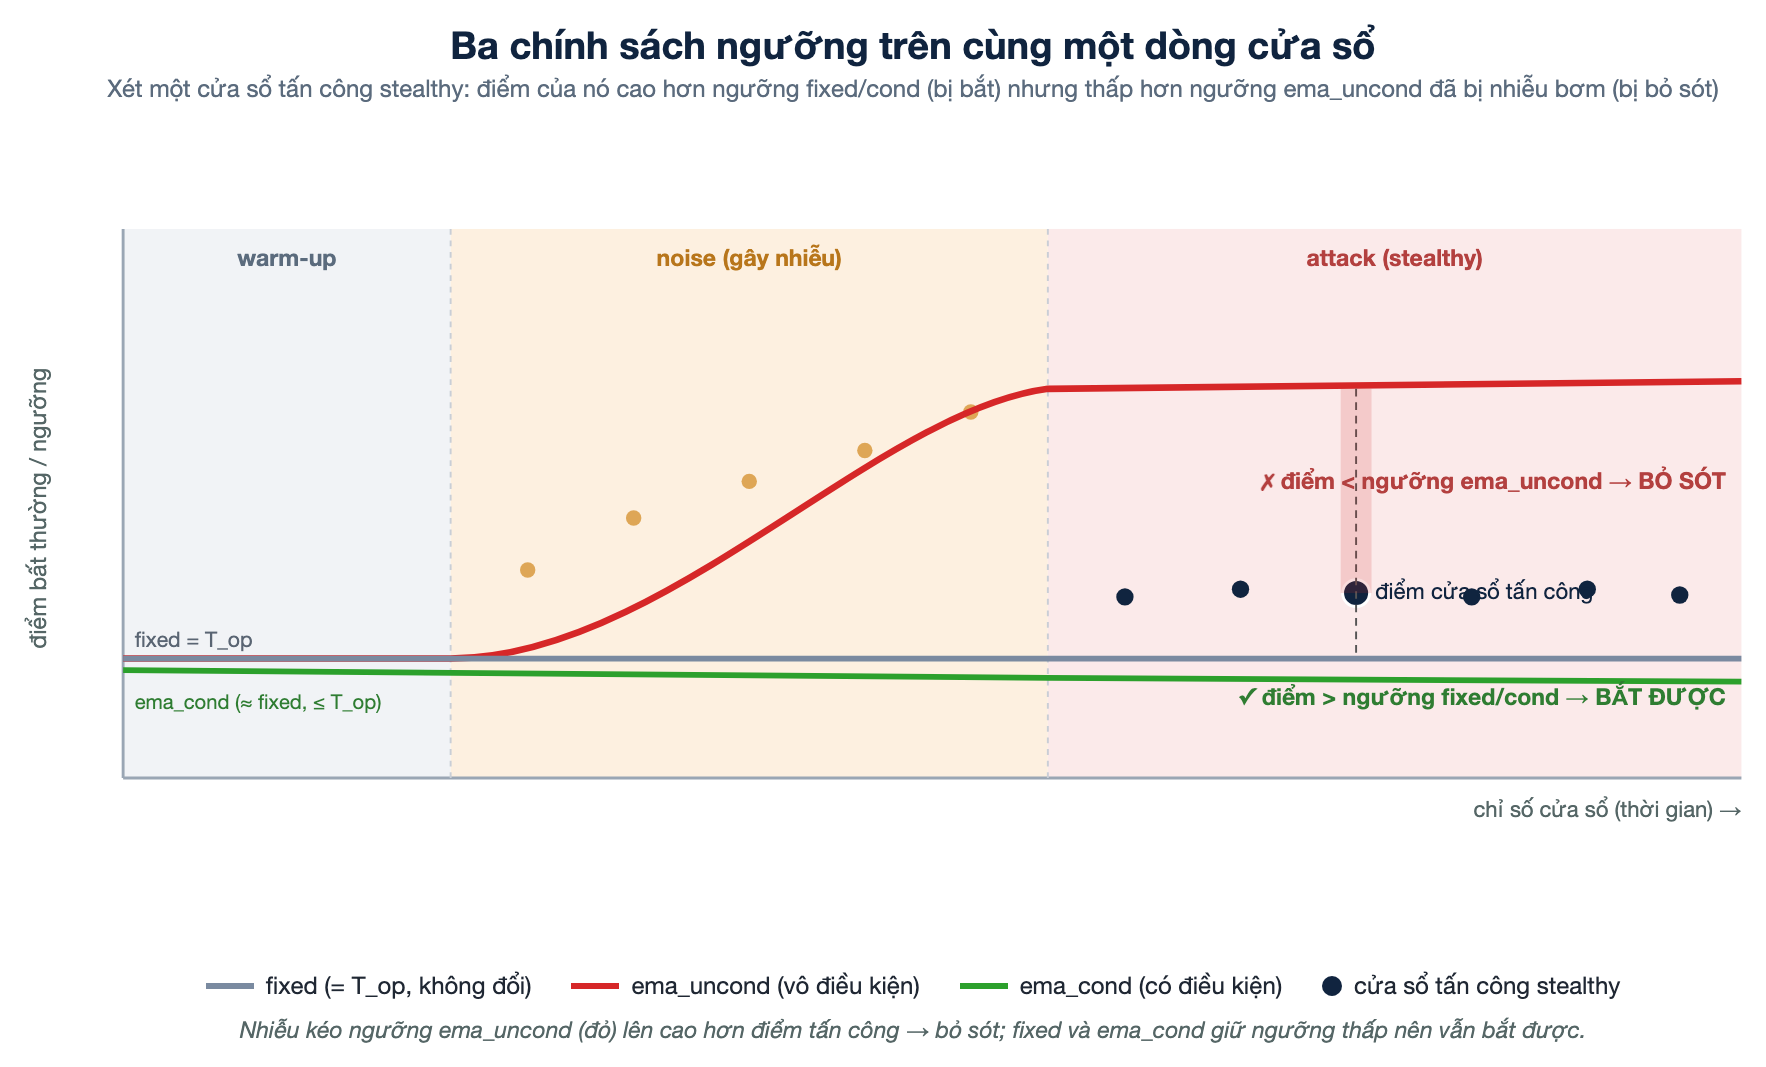
\includegraphics[width=\textwidth]{figures/fig_policy.png}
\caption{Minh hoạ khái niệm ba chính sách ngưỡng trên dòng warm-up$\to$noise$\to$attack: nhiễu kéo \texttt{ema\_uncond} vượt lên trên các điểm tấn công stealthy (vùng evasion), trong khi \texttt{fixed} và \texttt{ema\_cond} vẫn ở dưới nên bắt được.}
\label{fig:policy}
\end{figure}

\subsection{Biến số, chỉ số và phương pháp thống kê}
Bảng~\ref{tab:metrics} định nghĩa các biến số và chỉ số kèm cách đo cụ thể. Mỗi quan sát thống kê là một \textit{trial} (một dòng cửa sổ độc lập), không phải từng cửa sổ riêng lẻ — nhờ vậy các phép kiểm định không bị thổi phồng mức ý nghĩa (tránh \textit{pseudoreplication}).

\begin{table}[ht]
\caption{Biến số và chỉ số.}
\label{tab:metrics}
\centering
\begin{tabular}{@{}p{3.6cm}p{8.4cm}@{}}
\toprule
\textbf{Ký hiệu} & \textbf{Định nghĩa} \\
\midrule
Cường độ nhiễu (IV) & $\{$none, moderate, high$\}$ — pod đồng trú sinh tải lành tính tăng dần \\
Attack class (factor) & $\{$stealthy (lén), loud (ồn)$\}$ \\
Recall & tỷ lệ cửa sổ tấn công có $A>T$ \\
FPR & tỷ lệ cửa sổ lành tính có $A>T$ \\
AUC-ROC / AP & năng lực phân tách benign/attack, độc lập ngưỡng \\
$T_{\text{EMA}}(t)$ & giá trị dynamic threshold theo thời gian \\
Evasion & cửa sổ tấn công bị bỏ sót dưới EMA \textit{nhưng} bị bắt dưới fixed threshold $T_{op}$ \\
\bottomrule
\end{tabular}
\end{table}

Vì mỗi trial lấy mẫu ngẫu nhiên nên recall dao động giữa các lần chạy; báo cáo dùng kiểm định thống kê để xác nhận khác biệt quan sát được là \textit{thật} chứ không do ngẫu nhiên — nếu giá trị $p$ nhỏ hơn mức ý nghĩa $\alpha=0{,}05$ thì bác bỏ H0. Với mỗi tổ hợp \textit{loại tấn công $\times$ cường độ nhiễu}, báo cáo chạy 40 trial độc lập và dùng ba phép kiểm định, mỗi phép trả lời một câu hỏi:
\begin{itemize}[leftmargin=1.2cm]
\item \textbf{Bootstrap 95\% CI} — recall thực dao động trong khoảng nào (độ tin cậy của con số);
\item \textbf{Kruskal--Wallis và Spearman} — recall có giảm đều khi nhiễu tăng không, và giảm mạnh đến đâu (kiểm định xu hướng, H1a);
\item \textbf{Wilcoxon ghép cặp} — trên \textit{cùng} một dòng dữ liệu, \texttt{fixed} có bắt được nhiều hơn \texttt{ema\_uncond} không, qua đó khẳng định evasion là do cơ chế ngưỡng chứ không do nguyên nhân khác (H1b).
\end{itemize}
Do các trial lấy mẫu \textit{có hoàn lại} từ pool hữu hạn, các giá trị $p$ nên được đọc như chỉ báo mạnh, không phải sai số tuyệt đối chặt chẽ.

%% ===================== 4. THIẾT LẬP =====================
\section{Thiết lập thực nghiệm}\label{sec:setup}

Thí nghiệm gồm hai bước, theo loại hình Applied Experimentation (Mục~\ref{sec:method}). Bước thứ nhất tái lập một bộ phát hiện kiểu DeSFAM (VAE + Isolation Forest, huấn luyện normal-only) trên dữ liệu thực DongTing và đánh giá năng lực phát hiện (RQ1). Bước thứ hai, trên chính dòng anomaly score của bộ phát hiện ấy, dựng một thí nghiệm đối kháng có kiểm soát: thao tác cường độ nhiễu của noisy neighbor và đối chứng ba chính sách ngưỡng trên \textit{cùng} một dòng dữ liệu (RQ2). Toàn bộ được thực hiện trên một pipeline ba phase tách biệt (train / calibrate / test rời rạc) nhằm loại rò rỉ dữ liệu. Các tiểu mục dưới đây trình bày lần lượt: dữ liệu, bộ phát hiện và trích xuất đặc trưng, mô hình mối đe doạ và hàng xóm gây nhiễu, và cuối cùng là quy trình ba phase cùng giao thức thí nghiệm.

\subsection{Dữ liệu}
Báo cáo sử dụng tập DongTing~\cite{dongting2023} ở dạng đã mã hoá (chuỗi system call ID theo bảng kernel 5.17): 5.105 chuỗi lành tính cho training, 656 chuỗi lành tính cho calibration và đánh giá, 6.436 chuỗi tấn công cho đánh giá. Đây là dữ liệu system call \textit{thực}, không phải dữ liệu tổng hợp.

\subsection{Bộ phát hiện và trích xuất đặc trưng}
\subsubsection{Bộ lọc sensor-alphabet: cơ chế, lý do và độ phủ}
Báo cáo áp dụng \textit{sensor-alphabet filter} (bảng chữ cái cảm biến) — chỉ giữ lại 24 system call liên quan an ninh (\texttt{execve, clone, setuid/setgid/capset, openat, unlinkat, renameat2, mount, unshare, setns, pivot\_root, socket, connect, bind, mprotect, mmap, prctl, memfd\_create, splice, ptrace, init/finit\_module, bpf}) — \textit{trước khi} windowing (độ dài 10, bước 2). Nhóm này chỉ chiếm $\sim 20\%$ system call ở chuỗi lành tính và $\sim 10\%$ ở chuỗi tấn công, song lại \textit{tập trung} tín hiệu privilege escalation.

Việc lọc trước khi windowing là cần thiết vì nhiều lý do hội tụ. Trước hết, nó \textit{tập trung tín hiệu và chống dilution}: dấu hiệu privilege escalation tập trung ở một nhóm nhỏ system call đặc quyền, trong khi workload lành tính bị áp đảo bởi \texttt{read/write/close/futex}; nếu đưa toàn bộ không gian system call vào, các call đặc quyền hiếm bị pha loãng đến mức mô hình normal-only không còn phân tách được benign với attack — thực nghiệm xác nhận điều này khi AUC tăng từ $0{,}504$ (không filter, gần như ngẫu nhiên) lên $0{,}832$ (có filter). Thứ hai, nó \textit{đồng bộ giữa huấn luyện và vận hành}: TracingPolicy của Tetragon khi triển khai chỉ trace đúng nhóm system call an ninh này, nên feature space lúc huấn luyện (trên DongTing) trùng khớp với tín hiệu cảm biến lúc vận hành. Thứ ba, nó \textit{giảm chi phí xử lý}: \texttt{read/write/futex} là các system call có tần suất cao nhất, loại bỏ chúng giúp giảm mạnh khối lượng tính toán, phù hợp với mục tiêu overhead $<1\%$ của DeSFAM. Cuối cùng, việc dùng binary presence trên một tập đặc quyền được tuyển chọn khiến kẻ tấn công khó \textit{pha loãng} tín hiệu bằng cách bơm thêm system call lành tính.

Tập 24 system call này được tuyển chọn để bao trọn các system call \textit{điều phối ranh giới đặc quyền}:
\begin{itemize}[leftmargin=1.2cm,itemsep=1pt]
\item đổi định danh / capability: \texttt{setuid, setgid, capset, prctl};
\item thao tác namespace--mount (container escape): \texttt{unshare, setns, pivot\_root, mount};
\item injection / tracing tiến trình: \texttt{ptrace}; nạp mã kernel: \texttt{init\_module, finit\_module, bpf};
\item execution: \texttt{execve, clone}; truy cập tệp nhạy cảm: \texttt{openat, unlinkat, renameat2};
\item memory permission: \texttt{mprotect, mmap, memfd\_create}; di chuyển dữ liệu: \texttt{splice}; network: \texttt{socket, connect, bind}.
\end{itemize}
Mọi kỹ thuật privilege escalation (TA0004) và container escape đều phải đi qua ít nhất một trong các ``kernel choke point'' này, nên 24 system call là \textit{đủ phủ} cho lớp tấn công được nghiên cứu. Bằng chứng định lượng: detector đạt AUC $0{,}832$, xấp xỉ mức DeSFAM-test ($\approx 0{,}835$), chỉ với feature space dựa trên 24 system call này. \textit{Giới hạn (xem Mục~\ref{sec:discuss}):} đây là một tập được tuyển chọn theo định hướng an ninh (khớp với TracingPolicy của Tetragon khi triển khai) chứ không nhằm liệt kê đầy đủ; một tấn công hoạt động hoàn toàn qua các system call ngoài tập (ví dụ \texttt{io\_uring} hoặc kênh data-only) sẽ không được quan sát — vì vậy mở rộng sensor alphabet là một hướng phát triển.

\subsubsection{Trích xuất đặc trưng}
Mỗi cửa sổ trượt (độ dài tối đa 10, chỉ gồm system call thuộc sensor alphabet 24 phần tử) được biểu diễn thành một feature vector 42 chiều, ghép từ ba khối (minh hoạ ở Hình~\ref{fig:fe}):
\begin{itemize}[leftmargin=1.2cm,itemsep=2pt]
\item \textbf{Tần suất (24 chiều):} tỷ lệ xuất hiện của mỗi system call trong alphabet, tính bằng số lần xuất hiện chia cho độ dài cửa sổ.
\item \textbf{Binary presence (15 chiều):} với 15 system call đặc quyền \textit{hiếm} (setuid/setgid/capset, unshare, setns, pivot\_root, mount, ptrace, init/finit\_module, bpf, memfd\_create, splice, renameat2, unlinkat), mỗi chiều chỉ ghi nhận \textit{có hay không} xuất hiện ($1$/$0$), thay vì đếm tần suất. Cách này nhằm \textbf{chống dilution}: một \texttt{ptrace} đơn lẻ trong một cửa sổ đầy \texttt{openat} vẫn ``lật bit'', trong khi tần suất sẽ làm chìm tín hiệu hiếm này.
\item \textbf{Thống kê (3 chiều):} entropy của phân phối tần suất, tỷ lệ số system call khác nhau trên 24, và tần suất lớn nhất — phản ánh mức độ đa dạng và tập trung của cửa sổ.
\end{itemize}
Toàn bộ vector được chuẩn hoá bằng RobustScaler (theo khoảng phân vị $p1$–$p99$), \textit{fit chỉ trên} cửa sổ normal-train. Quá trình huấn luyện và vận hành dùng \textit{cùng} một feature space 42 chiều — điều kiện để mô hình học trên DongTing áp dụng được cho dòng cửa sổ ở phase test/triển khai.

\begin{figure}[ht]
\centering
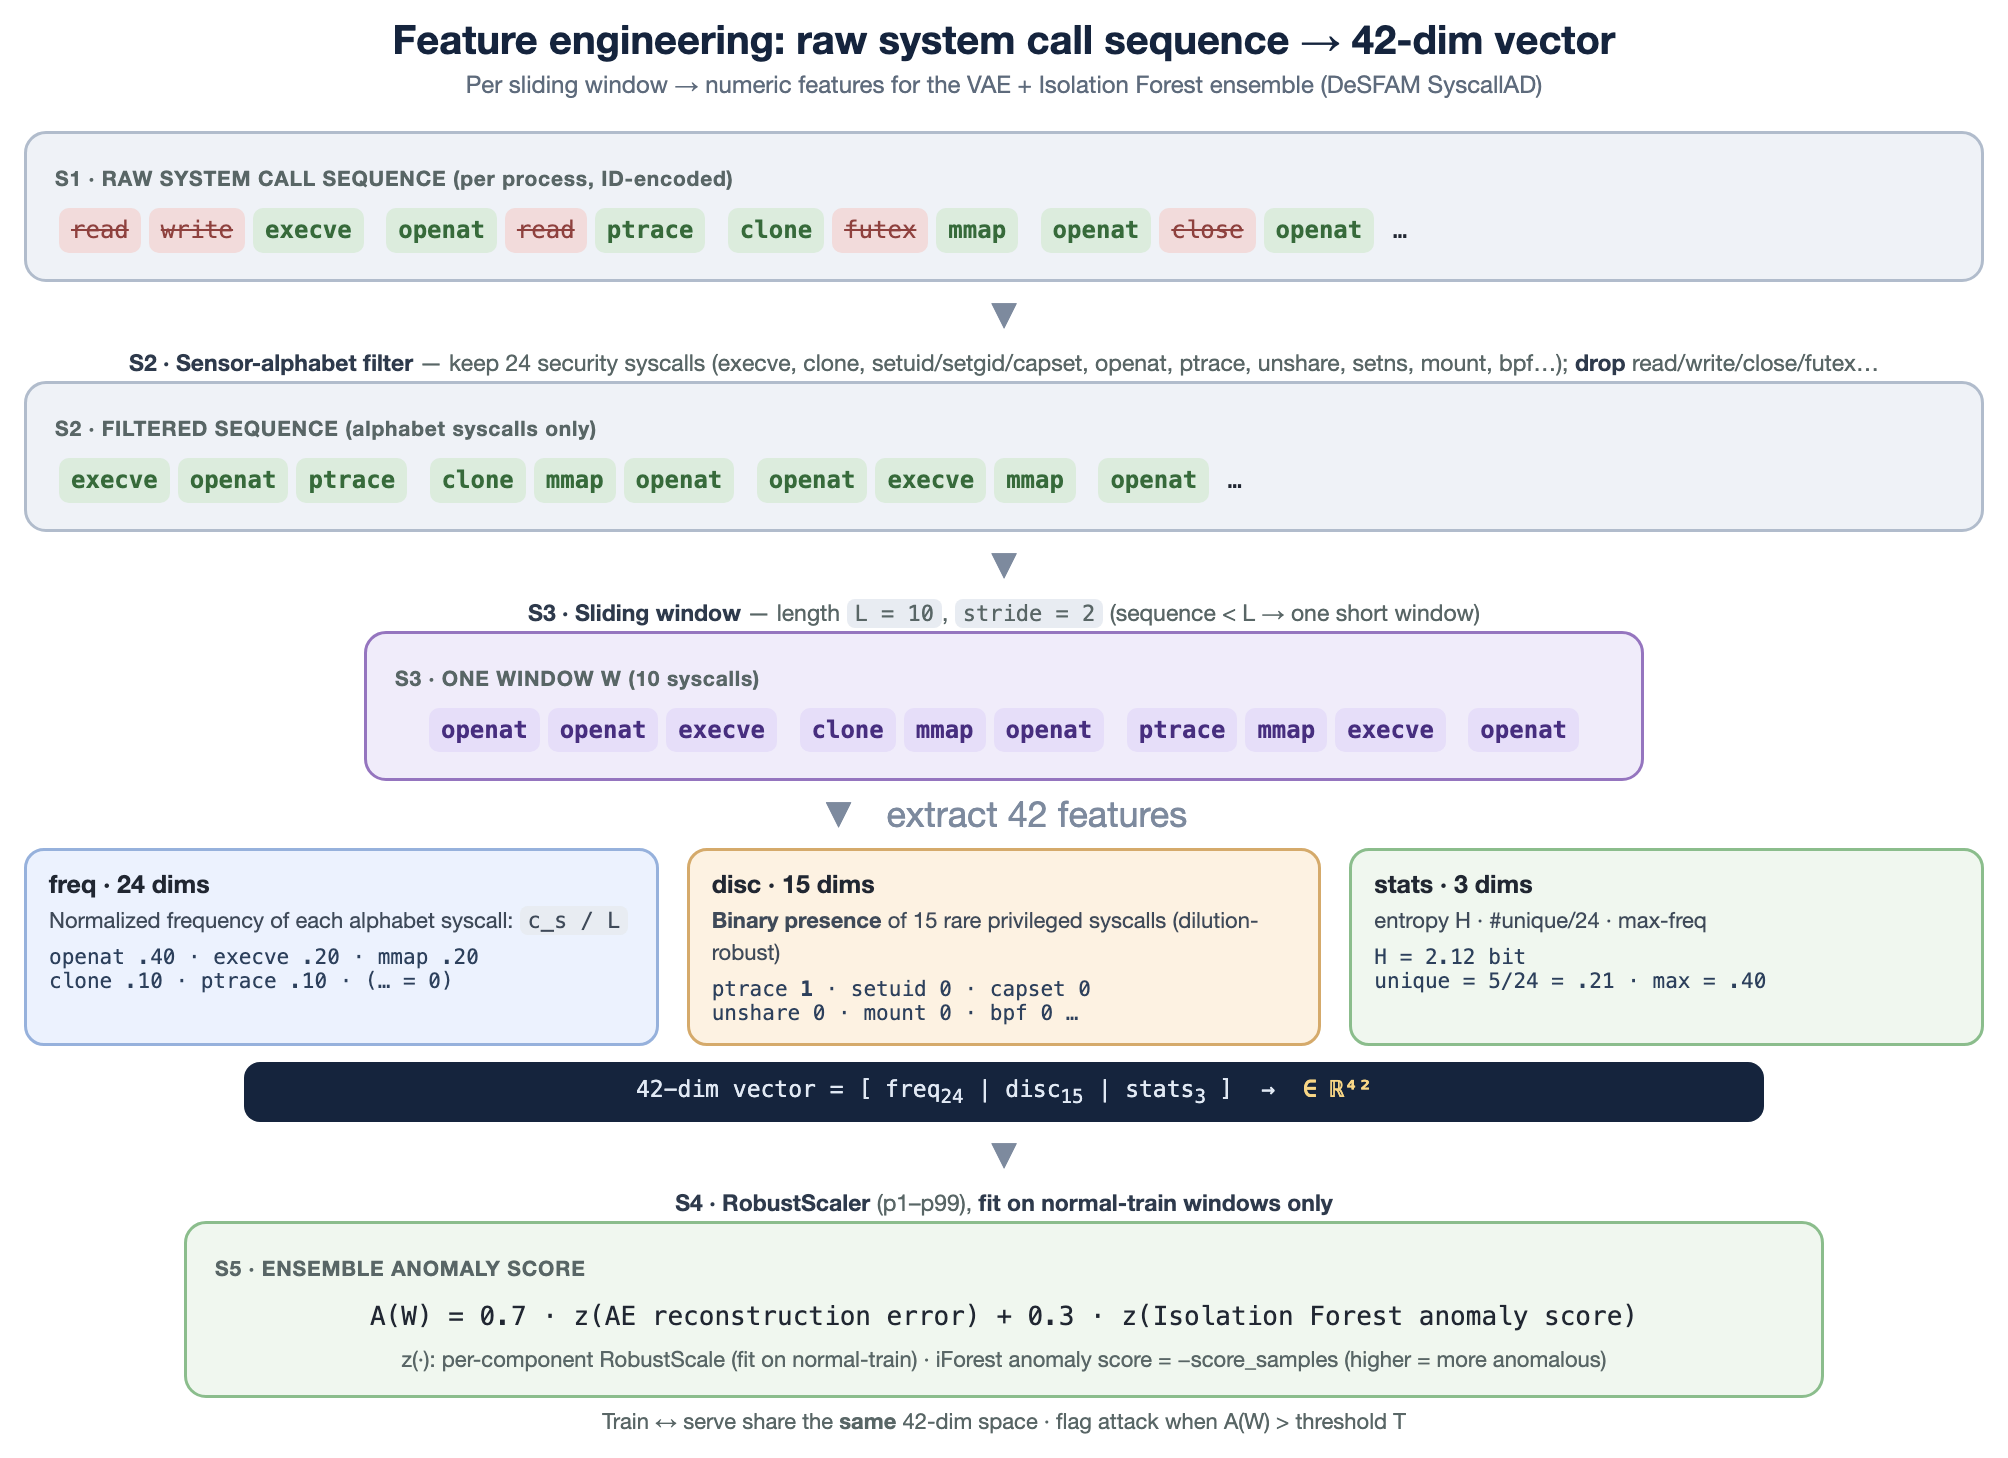
\includegraphics[width=0.96\textwidth]{figures/fig_features.png}
\caption{Quy trình trích xuất đặc trưng (ví dụ một cửa sổ).}
\label{fig:fe}
\end{figure}

\subsubsection{Bộ phát hiện (VAE + Isolation Forest)}
Bộ phát hiện được huấn luyện theo chế độ \textit{normal-only}, đúng theo thiết kế DeSFAM: một \textit{Variational Autoencoder} (VAE) và một Isolation Forest. VAE được cài bằng TensorFlow/Keras (encoder $42\to24\to$ latent $6$; huấn luyện Adam, 40 epoch); điểm bất thường của VAE là sai số tái tạo (reconstruction error) tính từ $z=\mu$. VAE ở đây được dựng lại theo \textit{kiến trúc} mô tả trong DeSFAM và huấn luyện lại trên DongTing; báo cáo không sử dụng mô hình đã huấn luyện sẵn (trọng số gốc) vì công trình gốc không phát hành chúng. Điểm của hai mô hình được RobustScale rồi hợp nhất theo trọng số $0{,}7/0{,}3$ thành anomaly score ensemble:
\[
A(W)=0{,}7\,z\big(\lVert g(\tilde{\mathbf{x}})-\tilde{\mathbf{x}}\rVert^2\big)+0{,}3\,z\big(-\mathrm{iForest}(\tilde{\mathbf{x}})\big),
\]
với $g$ là VAE (giải mã từ $z=\mu$) và $z(\cdot)$ là RobustScale từng thành phần (fit trên normal-train). Ngưỡng khởi tạo $T_0$ đặt tại phân vị $99{,}5$ của anomaly score lành tính (các mức ngưỡng $T_0/T_{op}/T_{\min}$ đã trình bày ở Mục~\ref{sec:method}).

\subsection{Mô hình mối đe doạ và hàng xóm gây nhiễu}
Kẻ tấn công được giả định đã có chỗ đứng trong một pod (post-exploitation) và thực hiện các kỹ thuật privilege escalation / container escape. Tấn công \textit{loud} (ồn) dùng nhiều system call đặc quyền dồn dập (anomaly score rất cao, $>$ phân vị $99{,}9$ lành tính); tấn công \textit{stealthy} (lén) rải mỏng (anomaly score chỉ vừa vượt operating point). \textit{Noisy neighbor} là một pod đồng trú sinh tải lành tính hỗn loạn (memory allocation, CPU, I/O), được mô hình hoá bằng các cửa sổ lành tính \textit{thực} của DongTing lấy theo dải phân vị anomaly score tăng dần: none ($\le$ phân vị 50), moderate (50--90), high ($>$ phân vị 90). Operating point $T_{op}$ đặt tại phân vị $95$ của anomaly score lành tính (FPR $\approx 5\%$); sàn EMA $T_{\min}$ đặt tại phân vị $50$.

\subsection{Quy trình ba phase và giao thức thí nghiệm}
\subsubsection{Ba phase tách biệt (đảm bảo độ tin cậy)}
Để loại bỏ rò rỉ (leakage) giữa calibration và đánh giá, pipeline được tách thành ba phase trên các tập dữ liệu \textit{rời rạc} (Hình~\ref{fig:pipeline}):
\begin{itemize}[leftmargin=1.2cm]
\item \textbf{Phase 1 — Training:} fit scaler, VAE, Isolation Forest và các component scaler \textit{chỉ} trên cửa sổ lành tính của tập train (50.877 cửa sổ), không nhiễm dữ liệu tấn công.
\item \textbf{Phase 2 — Calibration:} đặt các ngưỡng $T_0/T_{op}/T_{\min}$ cùng các mốc phân vị xác định dải noise và dải attack \textit{chỉ} trên tập calibration (½ benign-val + ½ attack).
\item \textbf{Phase 3 — Test:} chấm điểm, báo cáo AUC/AP và dựng các dòng thí nghiệm trên tập test \textit{rời rạc} với tập calibration (nửa còn lại).
\end{itemize}
Vì $\text{CAL}\cap\text{TEST}=\varnothing$, không có ngưỡng hay mốc phân vị nào được fit trên chính các cửa sổ dùng để đánh giá — qua đó loại bỏ calibration leakage và tăng độ tin cậy của kết luận.

\begin{figure}[ht]
\centering
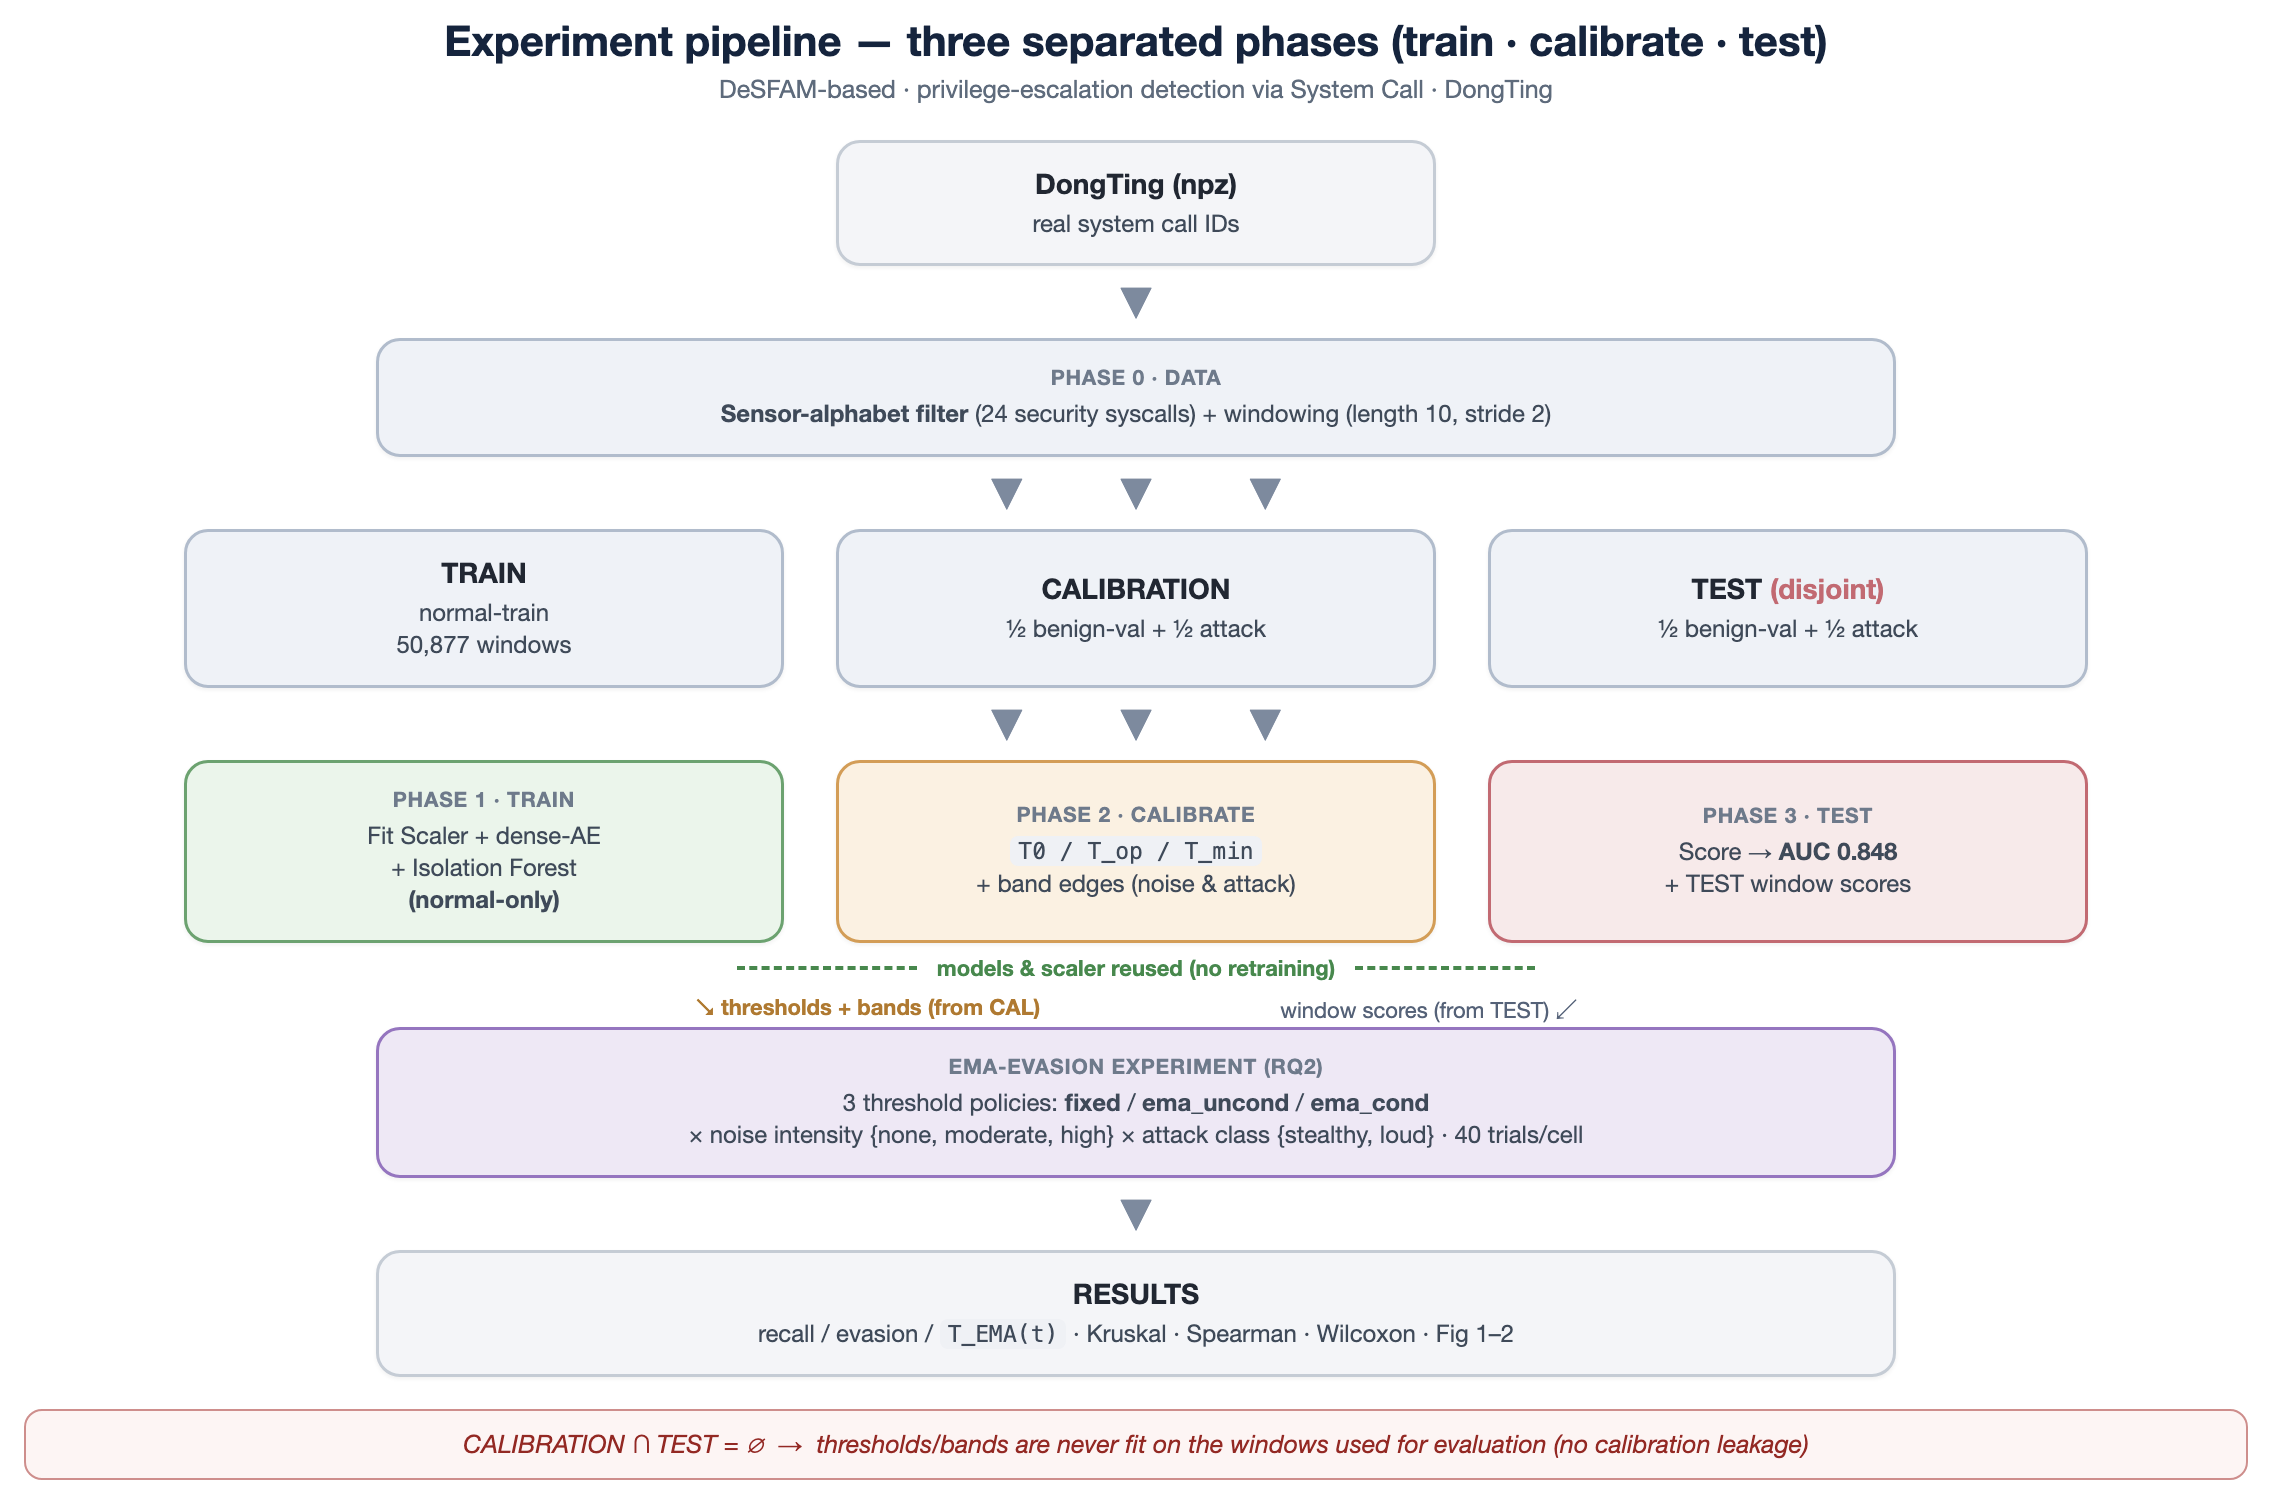
\includegraphics[width=0.92\textwidth]{figures/fig0_pipeline.png}
\caption{Pipeline thực nghiệm ba phase tách biệt ($\text{CAL}\cap\text{TEST}=\varnothing$).}
\label{fig:pipeline}
\end{figure}

\subsubsection{Cách tiến hành mỗi lượt thử (trial)}
Một \textit{trial} là một lượt chạy thí nghiệm độc lập trên một dòng cửa sổ tự dựng. Mỗi trial gồm các bước:
\begin{enumerate}[leftmargin=1.4cm]
\item \textbf{Dựng dòng cửa sổ TEST theo thứ tự thời gian:} warm-up (50 cửa sổ lành tính) $\to$ noise (150 cửa sổ, theo cường độ none/moderate/high) $\to$ attack (30 cửa sổ, theo loại stealthy/loud) — mô phỏng kịch bản vận hành bình thường, rồi hàng xóm bơm nhiễu, rồi tấn công xảy ra.
\item \textbf{Chạy cả ba chính sách ngưỡng} (\texttt{fixed}, \texttt{ema\_uncond}, \texttt{ema\_cond}) trên \textit{cùng} dòng cửa sổ đó để so sánh ghép cặp (cùng dữ liệu, chỉ khác chính sách).
\item \textbf{Lặp lại 40 trial} cho mỗi tổ hợp (loại tấn công $\times$ cường độ nhiễu).
\end{enumerate}
Cửa sổ trong mỗi trial được lấy mẫu \textit{có hoàn lại} từ các pool TEST hữu hạn (noise: $\approx$2530/1507/402 cửa sổ cho none/moderate/high; attack: $\approx$965 stealthy, $\approx$2883 loud); vì pool hữu hạn nên các trial không hoàn toàn độc lập — do đó CI bootstrap nên được đọc như chỉ báo, không phải sai số chuẩn chặt chẽ. Chi tiết tái lập ở Phụ lục~\ref{sec:repro}.

%% ===================== 5. KẾT QUẢ =====================
\section{Kết quả}\label{sec:results}

\subsection{RQ1 — Năng lực phát hiện trên DongTing}
Bảng~\ref{tab:detector} cho thấy sensor-alphabet filter nâng AUC từ $0{,}504$ (không filter — gần như ngẫu nhiên) lên $\mathbf{0{,}832}$ \textit{trên tập test rời rạc} — xấp xỉ mức DeSFAM-test công bố ($\approx0{,}835$), khẳng định tín hiệu privilege escalation tập trung ở nhóm system call đặc quyền và rằng đặc trưng binary presence trên các system call hiếm đóng vai trò quyết định. Recall@$T_0$ thấp ($0{,}005$) là hệ quả của việc $T_0$ rất khắt khe (phân vị $99{,}5$) và phù hợp với đặc tính recall thấp của các mô hình normal-only trên DongTing. Chính sự chồng lấn giữa phân phối anomaly score lành tính và tấn công đã tạo nên một \textit{dải stealthy} thực — gồm các tấn công có điểm chỉ vừa vượt ngưỡng vận hành — để khảo sát ở RQ2.

\begin{table}[ht]
\caption{Chất lượng detector trên DongTing.}
\label{tab:detector}
\centering
\begin{tabular}{@{}lcccc@{}}
\toprule
\textbf{Cấu hình feature} & \textbf{AUC} & \textbf{AP} & \textbf{Recall@$T_0$} & \textbf{FPR@$T_0$} \\
\midrule
Không filter (ablation, top-20 freq) & 0{,}504 & 0{,}971 & 0{,}001 & 0{,}006 \\
\textbf{Sensor-alphabet filter (TEST)} & \textbf{0{,}832} & 0{,}967 & 0{,}005 & 0{,}001 \\
\bottomrule
\end{tabular}
\par\smallskip{\footnotesize AP cao một phần do attack chiếm $\approx 91\%$ cửa sổ trong tập đánh giá (base rate cao); cần đọc kèm AUC/recall.}
\end{table}

\subsection{RQ2 — Threshold-inflation evasion}
Bảng~\ref{tab:full} trình bày recall đầy đủ theo ba chính sách ngưỡng $\times$ ba mức cường độ nhiễu $\times$ hai loại tấn công.

\begin{table}[ht]
\caption{Recall theo chính sách ngưỡng và cường độ nhiễu.}
\label{tab:full}
\centering
\begin{tabular}{@{}llccc@{}}
\toprule
\textbf{Attack class} & \textbf{Policy} & \textbf{none} & \textbf{moderate} & \textbf{high} \\
\midrule
stealthy & \texttt{fixed}      & 1{,}00 & 1{,}00 & 1{,}00 \\
stealthy & \texttt{ema\_uncond}& 1{,}00 & 1{,}00 & \textbf{0{,}258} \\
stealthy & \texttt{ema\_cond}  & 1{,}00 & 1{,}00 & 1{,}00 \\
\midrule
loud & \texttt{fixed}      & 1{,}00 & 1{,}00 & 1{,}00 \\
loud & \texttt{ema\_uncond}& 0{,}923 & 0{,}951 & 0{,}707 \\
loud & \texttt{ema\_cond}  & 1{,}00 & 1{,}00 & 1{,}00 \\
\bottomrule
\end{tabular}
\end{table}

\textbf{H1a (xu hướng).} Với \texttt{ema\_uncond}, recall của tấn công stealthy giảm theo cường độ nhiễu ($1{,}00 \to 1{,}00 \to 0{,}258$). Kruskal--Wallis $H=87{,}4$ ($p=1{,}1\times10^{-19}$); Spearman $\rho=-0{,}74$ ($p=3{,}1\times10^{-22}$) — \textit{bác bỏ} H0. Hình~\ref{fig:recall} minh hoạ bằng box-plot.

\textbf{Mức inflation của ngưỡng.} Giá trị EMA threshold trung bình tại thời điểm tấn công tăng theo cường độ nhiễu đối với tấn công stealthy: $\approx 0{,}53$ (none) $\to 0{,}86$ (moderate) $\to 10{,}9$ (high) — vượt $T_{op}=8{,}79$ ở mức cao (Hình~\ref{fig:traj}), đúng với tốc độ tiệm cận đã dự đoán ở Mục~\ref{sec:method}. Tương quan dương giữa cường độ nhiễu và $T_{\text{EMA}}$ trực tiếp giải thích sự suy giảm recall.

\subsection{RQ2 — Evasion và vai trò của cập nhật có điều kiện}
Bảng~\ref{tab:rq2} (noise cao, tấn công stealthy): fixed threshold bắt $100\%$ cửa sổ; cập nhật vô điều kiện \texttt{ema\_uncond} (cách đọc theo nghĩa đen công thức~\eqref{eq:ema}) chỉ còn $25{,}8\%$, tức \textbf{evasion $74{,}2\%$} (Wilcoxon $p=2{,}3\times10^{-7}$), khi ngưỡng bị inflate từ $T_{op}=8{,}79$ lên $\approx10{,}9$ tại thời điểm tấn công (đỉnh $\approx11{,}5$, Hình~\ref{fig:traj}). Đây là bằng chứng nhân quả: evasion chỉ xuất hiện khi ngưỡng được cập nhật vô điều kiện. Ngược lại, dạng cập nhật có điều kiện \texttt{ema\_cond} — \textit{chính là Algorithm 2 của DeSFAM} — giữ ngưỡng đơn điệu không tăng (giảm về sàn $\approx0{,}53$) và đạt \textbf{evasion $0\%$} ở \textit{mọi} điều kiện và \textit{cả hai} attack class. Nói cách khác, lỗ hổng chỉ phát sinh khi triển khai theo nghĩa đen công thức~\eqref{eq:ema}; Algorithm 2 vốn đã miễn nhiễm.

\begin{table}[ht]
\caption{Recall và evasion theo policy (noise cao, stealthy).}
\label{tab:rq2}
\centering
\begin{tabular}{@{}lccc@{}}
\toprule
\textbf{Policy} & \textbf{Recall} & \textbf{Evasion} & \textbf{$T$ lúc tấn công} \\
\midrule
\texttt{fixed} & 1{,}00 & --- & 8{,}79 \\
\texttt{ema\_uncond} (Eq.~\ref{eq:ema}) & \textbf{0{,}258} & \textbf{74{,}2\%} & 8{,}8 $\to$ 11{,}5 \\
\texttt{ema\_cond} (Algorithm 2) & 1{,}00 & \textbf{0{,}0\%} & $\approx0{,}53$ \\
\bottomrule
\end{tabular}
\end{table}

\textbf{Tính bất ổn nội tại của Eq.~\eqref{eq:ema}.} Bảng~\ref{tab:full} cho thấy hiện tượng phụ thuộc loại tấn công. Với tấn công \textit{loud} (điểm bất thường rất cao), ngay ở cột \textit{none} — không có noisy neighbor — \texttt{ema\_uncond} đã để lọt $\approx 8\%$ cửa sổ (recall $0{,}923$): điểm cực cao của \textit{chính các cửa sổ tấn công} tự bơm ngưỡng (self-inflation), chứng tỏ dạng cập nhật vô điều kiện bất ổn ngay cả khi không có đối thủ. Với tấn công \textit{stealthy}, hiện tượng này chưa xuất hiện ở mức nhiễu thấp (recall $1{,}00$ ở none và moderate) mà chỉ bộc lộ dưới nhiễu cao (recall $0{,}258$) — nghĩa là ở đây \textit{một noisy neighbor là điều kiện cần} để đẩy ngưỡng đủ cao gây evasion. Tóm lại, lỗ hổng nằm ở \textit{cập nhật vô điều kiện} (tích hợp mọi cửa sổ, kể cả cửa sổ điểm cao); dạng có điều kiện của Algorithm 2 (DeSFAM) miễn nhiễm cả hai trường hợp.

\begin{figure}[ht]
\centering
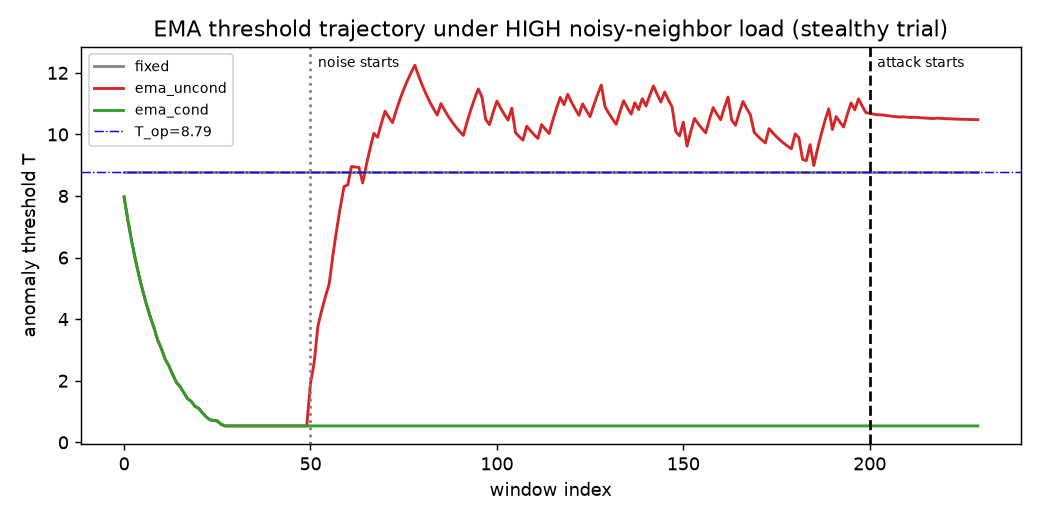
\includegraphics[width=0.92\textwidth]{figures/fig1_threshold.png}
\caption{Quỹ đạo ngưỡng $T$ trong một lượt thử nhiễu cao (tấn công stealthy). Khi nhiễu bắt đầu (cửa sổ 50), \texttt{ema\_uncond} (đỏ) bị kéo vọt lên \textit{trên} $T_{op}=8{,}79$ và duy trì ở mức cao suốt giai đoạn tấn công (từ cửa sổ 200) nên bỏ sót tấn công; \texttt{ema\_cond} (xanh) giảm về sàn $\approx0{,}5$ và giữ nguyên nên vẫn bắt được.}
\label{fig:traj}
\end{figure}

\begin{figure}[ht]
\centering
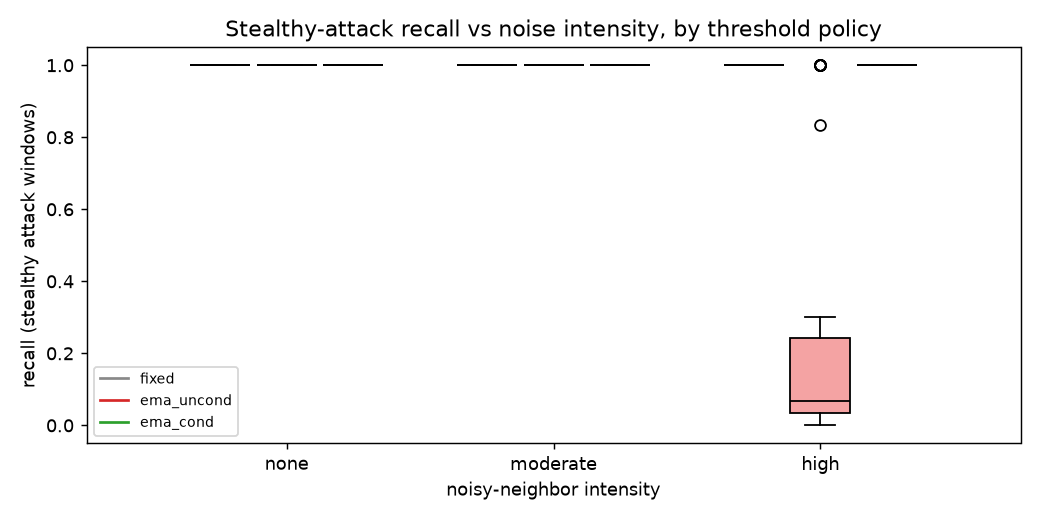
\includegraphics[width=0.92\textwidth]{figures/fig2_recall.png}
\caption{Recall của tấn công stealthy theo cường độ nhiễu, phân theo chính sách (box-plot trên 40 trial). Ở mức none/moderate cả ba chính sách đều đạt recall $1{,}0$; chỉ ở mức nhiễu cao, \texttt{ema\_uncond} (đỏ) sụt mạnh (trung vị $\approx0{,}06$), trong khi \texttt{fixed} và \texttt{ema\_cond} vẫn giữ $1{,}0$.}
\label{fig:recall}
\end{figure}

%% ===================== 6. THẢO LUẬN =====================
\section{Thảo luận}\label{sec:discuss}

Lỗ hổng đến từ \textit{cập nhật ngưỡng vô điều kiện} (cách đọc theo nghĩa đen công thức~\eqref{eq:ema}): tích hợp mọi cửa sổ, kể cả cửa sổ điểm cao, làm detector mất độ nhạy đúng vào lớp tấn công stealthy — vốn nguy hiểm và khó quan sát nhất (ví dụ container escape qua \texttt{nsenter}/\texttt{ptrace} rải mỏng). Quan trọng hơn, đối chiếu trực tiếp \textit{Algorithm 2} của DeSFAM cho thấy DeSFAM đặc tả cập nhật \textit{có điều kiện} (chỉ trên cửa sổ không bị gắn cờ) — vốn đã miễn nhiễm với lỗ hổng này. Vì vậy đóng góp của báo cáo không phải một cơ chế mới, mà là: (i) làm rõ sự \textit{thiếu nhất quán} ngay trong bài báo DeSFAM — công thức~\eqref{eq:ema} (vô điều kiện) so với Algorithm 2 (có điều kiện); và (ii) chứng minh bằng thực nghiệm rằng dạng cập nhật có điều kiện của Algorithm 2 là \textit{thiết yếu về an ninh} — một bản triển khai theo nghĩa đen công thức~\eqref{eq:ema} để lọt $74{,}2\%$ tấn công stealthy, trong khi Algorithm 2 đạt $0\%$.

Hệ quả vận hành: đội ngũ SOC nên (a) cập nhật ngưỡng \textit{chỉ} trên cửa sổ không bị gắn cờ (đúng theo Algorithm 2 của DeSFAM, không theo nghĩa đen công thức~\eqref{eq:ema}); và (b) giám sát chính quỹ đạo $T_{\text{EMA}}(t)$ như một tín hiệu an ninh, vì tải lành tính bất thường có thể ``làm điếc cảm biến'' (sensor blinding).

Về định vị, DeSFAM~\cite{desfam_original} báo cáo precision/recall $94\%/90\%$ và FedMon~\cite{fedmon2025} $94\%/91\%$, đều trên workload chuẩn không thù địch; cả hai chưa kiểm thử kịch bản nhiễu đối kháng, đồng thời cụ thể hoá thách thức \textit{non-IID} mà FedMon thừa nhận. Đóng góp của báo cáo không nhằm vượt các chỉ số này; việc detector tái lập đạt AUC $0{,}832$ (xấp xỉ DeSFAM-test) bảo đảm hiện tượng quan sát được không phải là tạo tác của một detector yếu.

Các mối đe doạ đến tính hợp lệ (construct / circularity / internal / external) được trình bày đầy đủ trong tài liệu phương pháp luận kèm theo.

%% ===================== 7. KẾT LUẬN =====================
\section{Kết luận và Hướng phát triển}\label{sec:concl}
Báo cáo áp dụng loại hình Applied Experimentation để (i) tái lập một detector kiểu DeSFAM (VAE + Isolation Forest) cho anomaly detection trên system call với dữ liệu DongTing thực (AUC $0{,}832$ sau sensor-alphabet filter) và (ii) định lượng hệ quả an ninh của việc cập nhật ngưỡng \textit{vô điều kiện}: khi triển khai theo nghĩa đen công thức EMA của DeSFAM, noise từ một noisy neighbor làm inflate ngưỡng và giúp $74{,}2\%$ tấn công stealthy đạt evasion, với xu hướng thống kê rõ rệt theo cường độ nhiễu ($\rho=-0{,}74$). Ngược lại, dạng cập nhật \textit{có điều kiện} mà chính \textit{Algorithm 2} của DeSFAM đặc tả vô hiệu hoá hoàn toàn vector này ($0\%$). Qua đó, báo cáo vạch ra một sự thiếu nhất quán trong chính bài báo DeSFAM (công thức EMA vô điều kiện so với Algorithm 2 có điều kiện) và chứng minh rằng quy tắc cập nhật có điều kiện là \textit{thiết yếu về an ninh}, không chỉ để giảm báo động giả. Hướng phát triển tiếp theo gồm: (1) xác thực online trên cụm K8s + Tetragon; (2) khảo sát ngưỡng theo từng container; và (3) bổ sung argument analysis cho system call nhằm chống tấn công stealthy triệt để hơn.


%% ===================== TÀI LIỆU THAM KHẢO =====================
\bibliographystyle{plain}
\bibliography{references}

%% ===================== PHỤ LỤC =====================
%% ===================== PHỤ LỤC =====================
\appendix
\section{Phụ lục — Tái lập kết quả}\label{sec:repro}
Mã nguồn tại \texttt{Experiment/}. VAE (TensorFlow/Keras) được huấn luyện trong Docker; thí nghiệm EMA chạy trên CPU trong vài phút:
\begin{verbatim}
cd Experiment && unzip -o ../DongTing_Official/npz.zip -d data/
# 1) detector VAE (TensorFlow/Keras) trong Docker -> scored_windows_vae.npz
docker run --rm -v "$PWD/..":/work -w /work/Experiment \
    training-train python vae_keras.py
# 2) thí nghiệm EMA (host venv: numpy/sklearn/scipy/pandas/matplotlib)
SCORED_NPZ=output/scored_windows_vae.npz OUT_SUFFIX=_vae \
    .venv/bin/python ema_evasion.py    # -> stats_vae.json, fig1/fig2_*_vae.png
# 3) ablation không filter (top-20 freq) -> AUC ~0.50
docker run --rm -v "$PWD/..":/work -w /work/Experiment \
    -e FILTER=0 training-train python vae_keras.py
\end{verbatim}
Tham số chốt: sliding window $10$/bước $2$; alphabet $24$ system call; feature $42$ chiều; ensemble $\alpha=0{,}7$; EMA $\beta=0{,}9$; $T_{op}$ = phân vị $95$, $T_{\min}$ = phân vị $50$ của anomaly score lành tính; $40$ trial/ô. Kết quả số lưu tại \texttt{output/\{detector\_report.json, stats.json, trials.csv, summary.csv\}}.


\end{document}
